\documentclass[11pt,a4paper]{article}
\usepackage[T1]{fontenc}
\usepackage{lmodern,microtype}
\usepackage[margin=24mm,headheight=14pt]{geometry}
\usepackage{amsmath,amssymb,amsthm,mathtools}
\usepackage{booktabs,graphicx,xcolor,enumitem,fancyhdr,xurl,tabularx,array}
\usepackage[numbers,sort&compress]{natbib}
\usepackage[colorlinks=true,linkcolor=plum,citecolor=plum,urlcolor=plum]{hyperref}
\definecolor{plum}{HTML}{6D3B70}
\definecolor{teal}{HTML}{267C78}
\definecolor{boxbg}{HTML}{F6F2F6}
\numberwithin{equation}{section}
\newtheorem{theorem}{Theorem}[section]
\newtheorem{lemma}[theorem]{Lemma}
\newtheorem{proposition}[theorem]{Proposition}
\newtheorem{corollary}[theorem]{Corollary}
\theoremstyle{definition}
\newtheorem{definition}[theorem]{Definition}
\newtheorem{example}[theorem]{Example}
\theoremstyle{remark}
\newtheorem{remark}[theorem]{Remark}
\newcommand{\KL}{D}
\newcommand{\E}{\mathbb E}
\newcommand{\R}{\mathbb R}
\newcommand{\etaKL}{\eta_{\mathrm{KL}}}
\newcommand{\one}{\mathbf 1}
\newcommand{\mra}{m_{\rho,\alpha}}
\newcommand{\ac}{\alpha_*}
\newcommand{\plain}[1]{\par\smallskip\noindent\textit{In plain words.} #1\par\smallskip}
\DeclareMathOperator{\supp}{supp}
\DeclareMathOperator{\Var}{Var}
\setlist{itemsep=3pt,topsep=5pt}
\setlength{\emergencystretch}{2em}
\pagestyle{fancy}
\fancyhf{}
\fancyhead[L]{\small Entropy contraction on complete bipartite graphs via reverse erasure}
\fancyfoot[C]{\thepage}
\renewcommand{\headrulewidth}{0.4pt}
\title{\textbf{Entropy contraction on complete bipartite graphs\\
via reverse erasure: only the rarest symbol matters}}
\author{Anonymous}
\date{Revised 3 November 2026}

\begin{document}
\maketitle
\thispagestyle{plain}
\begin{abstract}
Caputo, Chen, Gu and Polyanskiy conjectured that one step of the half-lazy
random walk on the complete bipartite graph \(K_{n,n}\) shrinks relative
entropy by at most the factor \(\log n/[2\log(2n)]\), with single vertices
as the only worst starting points. They proved the case \(n=3\) with
computer assistance. We prove the conjecture for every \(n\), and for
\(K_{m,n}\) with \(M=\max(m,n)\) in place of \(n\). The key observation is
that one step of this walk splits into two copies of a simple channel, the
Bayesian reverse of an erasure channel: keep the current symbol with
probability \(\alpha\), otherwise replace it by a fresh draw from a prior
\(\rho\). For this channel we show that the relative-entropy contraction
coefficient depends on the prior only through its smallest atom \(q\), at
every retention probability. Up to the sharp threshold
\(\alpha=q^{q/(1-q)}\) the coefficient is \(\log(1/q)/\log(1/(\alpha q))\),
which is a translation of a mean inequality of Gao; above the threshold
the worst inputs become full-support exponential tilts. Further
consequences are a rank-one weighted bipartite extension (which also settles
a numerical observation on the lazy star), an extension to block-reset
chains, and the exact one-way communication rate for agreement distillation
when the party holding the erased copy speaks.
\end{abstract}

\noindent\textbf{Keywords.} Strong data processing; relative entropy;
contraction coefficient; reverse erasure; Markov chains; complete bipartite
graph; weighted means; agreement distillation.

\medskip
\noindent\textbf{Status.} Unrefereed research candidate prepared with AI
assistance; see Section~\ref{sec:status}. Text CC0-1.0; code MIT.

\section{Introduction}\label{sec:intro}

\subsection{Why entropy contraction coefficients?}

Let \(K\) be a Markov kernel on a finite set and \(\pi\) a probability law
with full support. If a random state with law \(v\) is moved one step by
\(K\), its relative entropy from \(\pi K\) can only decrease. The
\emph{contraction coefficient} records the worst-case fraction that
survives:
\begin{equation}\label{eq:eta}
\etaKL(\pi,K)=\sup_{v\ne\pi}
\frac{\KL(vK\|\pi K)}{\KL(v\|\pi)},\qquad
\KL(v\|\pi)=\sum_x v_x\log\frac{v_x}{\pi_x}.
\end{equation}
All logarithms are natural unless stated otherwise, and \(0\log0=0\). The
reference law \(\pi\) is fixed throughout; maximising also over \(\pi\) is a
different problem \cite{ordentlich}. An \emph{extremiser} is a law
\(v\ne\pi\) at which the supremum in \eqref{eq:eta} is attained.

Inequalities of the form \(\KL(vK\|\pi K)\le c\,\KL(v\|\pi)\) are
\emph{strong data-processing inequalities}. They go back to Ahlswede and
G\'acs \cite{ahlswede}, and are surveyed in
\cite{raginsky,polyanskiywu}. In Markov-chain language, \(1-\etaKL(\pi,P)\)
is a one-step rate of entropy decay towards the stationary law \(\pi\). A
useful benchmark is the \emph{local} (\(\chi^2\)) coefficient, obtained by
letting \(v\) approach \(\pi\); for a reversible chain it is the square of
the second-largest absolute eigenvalue. The global coefficient
\eqref{eq:eta} is never smaller, and can be strictly larger; comparisons
between such coefficients are developed in \cite{makur,raginsky}.

\subsection{The conjecture, and why it was posed}

Caputo, Chen, Gu and Polyanskiy (CCGP) \cite{caputo} compare three ways of
measuring entropy decay: half-step, full-step and continuous-time. They
point out that, unlike the extremal functions for log-Sobolev-type
constants, extremal distributions for \(\etaKL\) can fail to have full
support. Their illustration for the full-step coefficient is the half-lazy
walk on \(K_{n,n}\): stay put with probability \(1/2\), otherwise jump to a
uniformly chosen vertex on the other side. (This is their lazy random walk,
Definition~2.4 in the authors' manuscript and Definition~4 in arXiv
v1.) In Example~4.4 (arXiv v1: Example~28) they report that numerical
computation suggests
\begin{equation}\label{eq:conjecture}
\etaKL(\pi,P)=\frac{\log n}{2\log(2n)},\qquad n\ge3,
\end{equation}
with equality only at point distributions. Their Proposition~4.5 (arXiv v1:
Proposition~29) proves \(n=3\) by a computer-assisted case analysis. The
text following the proof of Proposition~4.5 conjectures the statement for
all \(n\ge3\) and says that it is unclear how to prove it in general.

The point of the example is therefore \emph{which inputs are worst}, not how
fast the walk mixes. The walk on \(K_{n,n}\) has spectral gap \(1/2\); its
one-step entropy decay rate \(1-\etaKL\) lies between \(3/4\) (\(n=2\)) and
\(1/2\) (\(n\to\infty\)) for \(n\ge2\). Our results give no new mixing-time information
for this chain. What they do give is an exact constant, the exact set of
worst starting states (single vertices, the ``cold start''), and an explicit
family in which the global coefficient tends to \(1/2\) while the local
coefficient stays at \(1/4\).

\subsection{The idea in one paragraph}

Watch the walk from one side of the graph. With probability \(1/2\) a
walker on side \(A\) stays where it is; otherwise it leaves, and the walkers
arriving on side \(A\) from side \(B\) land at a fresh uniform vertex of
\(A\). So the conditional law on side \(A\) after one step is ``keep the old
symbol with some probability, otherwise draw a fresh one from the prior''.
That is the Bayesian reverse of an erasure channel. An erasure channel keeps
a symbol with probability \(\alpha\) and otherwise outputs the blank symbol
\(e\); its reverse sends a kept symbol to itself and fills a blank with a
fresh sample. Section~\ref{sec:bipartite} makes this exact: one step of the
half-lazy bipartite walk is a pair of reverse-erasure channels at retention
\(\alpha=1/2\), with one bookkeeping term that is paid only once. The whole
problem is thus reduced to computing the contraction coefficient of reverse
erasure, which Sections~\ref{sec:main}--\ref{sec:supercritical} do for
every prior and every retention probability.

\subsection{What is new and what is inherited}

Given Gao's weighted mean inequality \cite{gao03,gao09}, the conjecture
\eqref{eq:conjecture} itself needs only two ingredients: the uniform-prior
reverse-erasure coefficient at \(\alpha=1/2\) (Theorem~\ref{thm:phase} with
uniform \(\rho\), whose upper bound \emph{is} Gao's inequality) and the
two-part decomposition of Section~\ref{sec:bipartite}. We say this plainly
because the analytic core of the closed formula is not ours. The new content
is:
\begin{enumerate}[label=(\alph*)]
\item the reduction to the smallest atom for \emph{every} prior and
\emph{every} retention probability, including the regime with no closed
formula (Theorem~\ref{thm:reduction}, Proposition~\ref{prop:scalar});
\item the sharpness of the threshold, the complete equality analysis, and
the description of extremisers above it
(Theorems~\ref{thm:phase} and~\ref{thm:supercritical});
\item the two-part decomposition, which proves the conjecture, extends it to
unequal parts and rank-one cross weights, and settles the lazy star
\(K_{1,N}\), left as a numerical observation by Jadhav \cite{jadhav}
(Theorem~\ref{thm:bipartite}, Corollary~\ref{cor:star});
\item Section~\ref{sec:blockreset}, which extends the reduction to
block-reset chains, including arbitrary laziness, matrix powers, stars and
multipartite graphs;
\item the exact one-way agreement-distillation rate for a general prior
(Corollary~\ref{cor:agreement}), a general-prior form of the uniform binary
case evaluated by Zhao \cite{zhao}.
\end{enumerate}
The reverse binary-erasure channel and its usefulness as an SDPI example
appear in Weinberger and Shayevitz \cite{weinberger}. The complete uniform
binary coefficient is known: the high-retention branch follows from Nair and
Wang \cite{nair} and the low-retention branch is Zhao's
\cite[Theorem~3.5.4]{zhao}; Appendix~\ref{app:binary} recalls both. Our
bounded literature search (Section~\ref{sec:status}) found no earlier
statement of (a), of an all-\(n\) proof of \eqref{eq:conjecture}, or of a
non-uniform closed form for this channel. Priority remains subject to
specialist review.

\subsection{Results at a glance}

Table~\ref{tab:glance} lists the results in the order in which they are
proved. Here \(q\) is the smallest prior atom, \(\alpha\) the retention
probability, and \(\ac(q)=q^{q/(1-q)}\) the threshold.

\begin{table}[htbp]
\centering
\small
\renewcommand{\arraystretch}{1.25}
\begin{tabularx}{\linewidth}{@{}>{\raggedright\arraybackslash}p{2.55cm}X>{\raggedright\arraybackslash}p{2.75cm}l@{}}
\toprule
Result & In words & New or known & Proof\\
\midrule
Theorem~\ref{thm:reduction}, Proposition~\ref{prop:scalar} &
The reverse-erasure coefficient depends on the prior only through \(q\);
an exact one-variable test decides it at every \(\alpha\). &
New & \S\ref{sec:reduction}\\
Theorem~\ref{thm:phase} &
For \(\alpha\le\ac(q)\) the coefficient is
\(\log(1/q)/\log(1/(\alpha q))\), attained only at a rarest point input;
the threshold is sharp. &
Upper bound is Gao's inequality; sharpness and general-prior form new &
\S\ref{sec:phase}\\
Proposition~\ref{prop:local}, Theorem~\ref{thm:supercritical} &
Local coefficient \(\alpha\); above the threshold the worst inputs are
full-support exponential tilts. & New & \S\ref{sec:supercritical}\\
Theorem~\ref{thm:bipartite}, Corollary~\ref{cor:star} &
Half-lazy \(K_{m,n}\): \(\log M/[2\log(2M)]\), only point extremisers for
\(M\ge3\); rank-one weights; lazy star. &
Conjecture of \cite{caputo}; proof new & \S\ref{sec:bipartite}\\
Section~\ref{sec:blockreset} &
Coefficient of any block-reset chain equals that of a chain with at most
two states per block (laziness, powers, stars, multipartite graphs); values
there are computed numerically. & New & \S\ref{sec:blockreset}\\
Corollary~\ref{cor:agreement} &
Below the threshold, the exact one-way rate for agreement distillation is
\(\log(1/\alpha)/\log(1/(\alpha q))\). &
Uniform binary case known \cite{zhao}; general prior new &
\S\ref{sec:agreement}\\
\bottomrule
\end{tabularx}
\caption{Main results. ``New'' means that no earlier statement was found in
the bounded search described in Section~\ref{sec:status}.}
\label{tab:glance}
\end{table}

\begin{center}
\fcolorbox{plum}{boxbg}{\begin{minipage}{0.93\linewidth}
\smallskip
\textbf{Worked example: \(K_{3,3}\).}
The stationary law is uniform, \(\pi_x=1/6\). Start at a single vertex
\(x\). Then \(\KL(\delta_x\|\pi)=\log6\). After one step the walker is at
\(x\) with probability \(1/2\) and at each of the three opposite vertices
with probability \(1/6\), so
\[
\KL(\delta_xP\|\pi)=\tfrac12\log\frac{1/2}{1/6}+3\cdot\tfrac16\log1
=\tfrac12\log3,\qquad
\frac{\KL(\delta_xP\|\pi)}{\KL(\delta_x\|\pi)}=\frac{\log3}{2\log6}
\approx0.3066 .
\]
This is the value in \eqref{eq:conjecture} and in CCGP's
Proposition~4.5. In the reverse-erasure picture, the conditional prior on
each side is uniform with \(q=1/3\), the retention probability is
\(\alpha=1/2\), and \(1/2\le\ac(1/3)=3^{-1/2}\approx0.577\), so the closed
formula applies (Figure~\ref{fig:exact}, right). The local coefficient is
only \(1/4\).
\smallskip
\end{minipage}}
\end{center}

\begin{figure}[htbp]
\centering
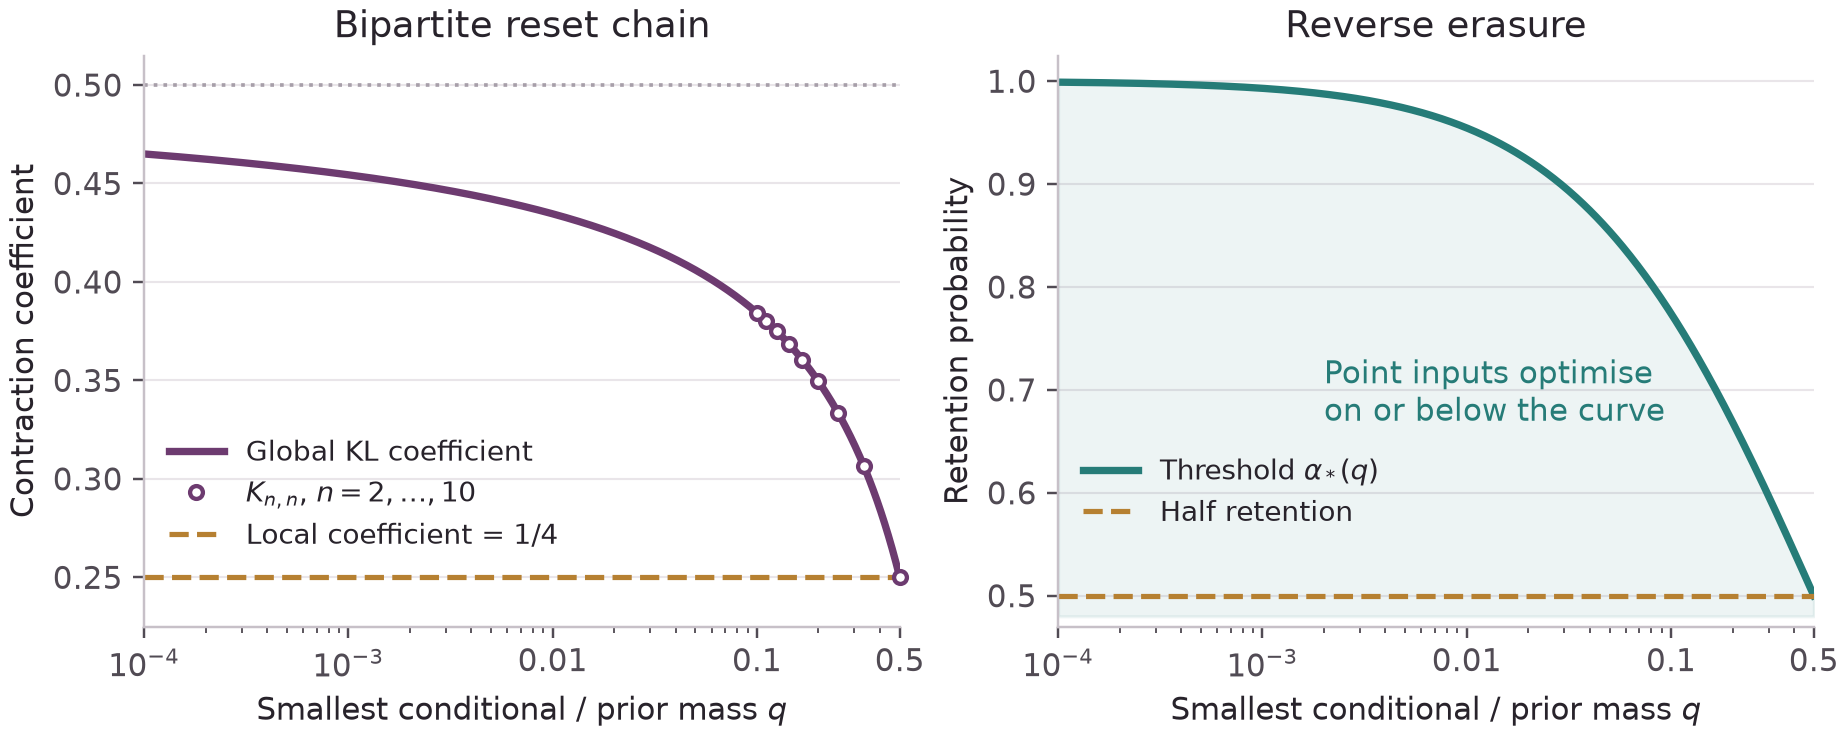
\includegraphics[width=\linewidth]{figures/exact_coefficients.png}
\caption{Exact formulas, not numerical fits. Left: the global coefficient
\(\log(1/q)/[2\log(2/q)]\) of a half-lazy bipartite reset chain rises
towards \(1/2\) as the smallest conditional mass \(q\) tends to zero; the
circles mark \(K_{n,n}\), \(q=1/n\), \(n=2,\ldots,10\). The local quadratic
coefficient stays at \(1/4\). Right: the reverse-erasure threshold
\(\ac(q)=q^{q/(1-q)}\). Retention \(1/2\) always lies on or below it, which
is why the bipartite walk is always in the regime with a closed formula.}
\label{fig:exact}
\end{figure}

\paragraph{Roadmap.}
Section~\ref{sec:main} sets up the channel and states the channel results.
Section~\ref{sec:reduction} proves the reduction to the smallest atom,
Section~\ref{sec:phase} the closed formula and its sharp threshold, and
Section~\ref{sec:supercritical} the regime above the threshold.
Section~\ref{sec:bipartite} proves the bipartite theorem and
Section~\ref{sec:blockreset} extends it to block-reset chains.
Section~\ref{sec:agreement} gives the communication application.
Section~\ref{sec:discussion} lists open problems and
Section~\ref{sec:status} records how the results were checked.
Appendices give the known uniform binary case, standard tensorisation and the
numerical diagnostics.

\subsection{Notation}

\begin{center}
\small
\renewcommand{\arraystretch}{1.2}
\begin{tabular}{@{}ll@{}}
\toprule
Symbol & Meaning\\
\midrule
\(\rho=(\rho_1,\ldots,\rho_n)\) & prior on the ordinary symbols, all \(\rho_i>0\), \(n\ge2\)\\
\(q=\min_i\rho_i\in(0,1/2]\) & smallest atom (``rarest symbol'')\\
\(\alpha\in(0,1)\) & retention probability of the erasure channel\\
\(R_\rho\) & reverse-erasure kernel \eqref{eq:reverse}\\
\(\mra=(\alpha\rho,1-\alpha)\) & input reference law, with \(\mra R_\rho=\rho\)\\
\(\eta(\rho,\alpha)\) & \(\etaKL(\mra,R_\rho)\), the coefficient studied here\\
\(c_0(q,\alpha)\) & \(\log(1/q)/\log(1/(\alpha q))\), the point-input ratio\\
\(\ac(q)\) & \(q^{q/(1-q)}\), the point-optimality threshold\\
\(p=1/c\) & dual exponent attached to a candidate coefficient \(c\)\\
\(G_\rho(z)\) & weighted geometric mean \(\prod_i z_i^{\rho_i}\)\\
\(H_{w,\alpha,p}(r)\) & one-variable dual test function \eqref{eq:H}\\
\(d(t\|s)\) & binary relative entropy\\
\bottomrule
\end{tabular}
\end{center}

\section{The reverse-erasure channel and the channel results}\label{sec:main}

\subsection{The channel}

Let \(\rho=(\rho_1,\ldots,\rho_n)\) be positive, \(n\ge2\). The
reverse-erasure kernel \(R_\rho\), from \([n]\cup\{e\}\) to \([n]\), is
\begin{equation}\label{eq:reverse}
R_\rho(i,\cdot)=\delta_i,\qquad R_\rho(e,\cdot)=\rho.
\end{equation}
For \(0<\alpha<1\), its input reference is
\begin{equation}\label{eq:reference}
\mra=(\alpha\rho_1,\ldots,\alpha\rho_n,1-\alpha),
\qquad \mra R_\rho=\rho.
\end{equation}
If \(X\sim\rho\) and \(E\) equals \(X\) with probability \(\alpha\) and \(e\)
otherwise, then \(E\sim\mra\) and \(R_\rho\) is the conditional law of \(X\)
given \(E\): the Bayesian reverse of the erasure channel. Set
\[
\eta(\rho,\alpha)=\etaKL(\mra,R_\rho),\qquad
q=\min_i\rho_i\in(0,1/2].
\]
Writing any input as \(v=(tu,1-t)\), with \(u\) a law on \([n]\) and
\(t\in[0,1]\) its ordinary mass, gives
\begin{equation}\label{eq:decomp}
vR_\rho=tu+(1-t)\rho,\qquad
\KL(v\|\mra)=d(t\|\alpha)+t\KL(u\|\rho).
\end{equation}

\begin{remark}[Where the channel appears]\label{rem:where}
(i) Composing the erasure channel with its reverse gives the lazy reset
kernel \(\alpha I+(1-\alpha)\one\rho^{\mathsf T}\): keep the symbol, or
resample it from \(\rho\). For uniform \(\rho\) this is the Potts channel
studied by Gu and Polyanskiy \cite{gupolyanskiy}, which therefore factors as
erasure followed by reverse erasure.
(ii) In sampling language, erasure is the ``down'' step and \(R_\rho\) the
``up'' (resampling) step of a down--up walk. For a product law
\(\rho^{\otimes N}\) with each coordinate erased independently,
tensorisation (Appendix~\ref{app:products}) shows that
\(\eta(\rho,\alpha)\) is exactly the KL contraction coefficient of the up
step of this block resampler, with the law of the erased configuration as
reference. For non-product targets the up step resamples from conditional
laws rather than from \(\rho\), so our results give only the product-measure
baseline. The proximal sampler \cite{proximal} is a continuous analogue
(noising forward, posterior denoising backward).
(iii) The coefficient \(\eta(\rho,\alpha)\) is the quantity \(s^*\)
attached to the pair (erased observation, clean symbol) in the
hypercontractivity language of Anantharam, Gohari, Kamath and Nair
\cite{anantharam}; Zhao's evaluation \cite[Theorem~3.5.4]{zhao} is stated in
that language.
\end{remark}

\subsection{The dual criterion and the test function \texorpdfstring{\(H\)}{H}}

A candidate coefficient \(c\in(0,1)\) can be tested without searching over
inputs. Put \(p=1/c\) and \(G_\rho(z)=\prod_i z_i^{\rho_i}\). By entropy
duality (Lemma~\ref{lem:duality}, proved in Section~\ref{sec:reduction}),
\(\eta(\rho,\alpha)\le c\) holds if and only if
\begin{equation}\label{eq:meancriterion}
\alpha\sum_i\rho_i z_i^p+(1-\alpha)G_\rho(z)^p
\le\left(\sum_i\rho_i z_i\right)^p
\qquad\text{for all }z\in[0,\infty)^n .
\end{equation}
This is an inequality between weighted means. It turns out that only test
vectors with one large coordinate matter. Evaluating
\eqref{eq:meancriterion} at \(z=(r,1,\ldots,1)\), with the large coordinate
at an atom of weight \(w\), and dividing the left side by the right side,
gives the one-variable function
\begin{equation}\label{eq:H}
H_{w,\alpha,p}(r)=
\frac{\alpha(wr^p+1-w)+(1-\alpha)r^{pw}}
{(wr+1-w)^p},\qquad r\ge1.
\end{equation}
We have \(H_{w,\alpha,p}(1)=1\). As \(r\to\infty\) the test vector, after
normalisation, concentrates on one coordinate; this limit corresponds to a
point input, and \(H_{w,\alpha,p}(\infty):=\lim_{r\to\infty}
H_{w,\alpha,p}(r)=\alpha w^{1-p}\).

\begin{definition}[Dual extremiser]\label{def:dualext}
Let \(p_*=1/\eta(\rho,\alpha)\). A \emph{dual extremiser} is a nonconstant
vector \(z\in[0,\infty)^n\setminus\{0\}\) at which \eqref{eq:meancriterion}
holds with equality for \(p=p_*\). It is \emph{positive} if every
coordinate is strictly positive.
\end{definition}

\subsection{Statements}

\begin{theorem}[Only the rarest symbol matters]\label{thm:reduction}
For every full-support finite prior \(\rho\) and every \(0<\alpha<1\),
\begin{equation}\label{eq:minreduction}
\eta(\rho,\alpha)=\eta((q,1-q),\alpha),\qquad q=\min_i\rho_i.
\end{equation}
\end{theorem}
\plain{Erasing and refilling forgets the same fraction of information,
in the worst case, for every prior whose rarest symbol has probability
\(q\). For example, the priors \((0.1,0.2,0.7)\) and \((0.1,0.9)\) have
exactly the same coefficient at every retention probability (although their
channels and extremisers differ).}

\begin{proposition}[Exact scalar criterion]\label{prop:scalar}
Let \(0<c<1\) and \(p=1/c\). Then \(\eta(\rho,\alpha)\le c\) if and only if
\[
H_{q,\alpha,p}(r)\le1\qquad\text{for every }r\in[1,\infty],
\]
where \(r=\infty\) means the point-input condition \(\alpha q^{1-p}\le1\).
Moreover, every positive dual extremiser has one large coordinate, located at
an atom of weight \(q\), and all its other coordinates equal.
\end{proposition}
\plain{To decide whether a number \(c\) bounds the coefficient, one only has
to check a function of one real variable.}

\begin{theorem}[Closed formula and sharp threshold]\label{thm:phase}
Define
\begin{equation}\label{eq:threshold}
\ac(q)=q^{q/(1-q)},\qquad
c_0(q,\alpha)=\frac{\log(1/q)}{\log(1/(\alpha q))}.
\end{equation}
\begin{enumerate}[label=(\roman*)]
\item If \(0<\alpha\le\ac(q)\), then
\begin{equation}\label{eq:atomic}
\eta(\rho,\alpha)=c_0(q,\alpha).
\end{equation}
Except when \(\rho=(1/2,1/2)\) and \(\alpha=1/2\), the extremisers are
exactly the point inputs \(\delta_i\) with \(\rho_i=q\).
\item If \(\alpha>\ac(q)\), then \(\eta(\rho,\alpha)>c_0(q,\alpha)\), so no
point input is an extremiser.
\end{enumerate}
\end{theorem}
\plain{Below the threshold the worst input simply announces the rarest symbol
with certainty. Above it, it pays to hedge with a little erasure mass:
the \(\epsilon\log\epsilon\) gain in output entropy beats the cost.}

For the uniform law on \(n\) symbols the threshold is \(n^{-1/(n-1)}\) and
\eqref{eq:atomic} reads \(\log n/\log(n/\alpha)\).

\begin{proposition}[Local versus global]\label{prop:local}
The local quadratic contraction coefficient of \(R_\rho\) at \(\mra\) is
\(\alpha\), and \(\eta(\rho,\alpha)<1\). Moreover
\(\eta(\rho,\alpha)>\alpha\) except when \(\rho=(1/2,1/2)\) and
\(\alpha\ge1/2\). (For the uniform binary prior, \(\eta>\alpha\) still holds
when \(\alpha<1/2\), by \eqref{eq:binary}.)
\end{proposition}
\plain{Small perturbations of the reference shrink by the factor \(\alpha\),
but large perturbations can shrink strictly less. For fixed \(\alpha\) and
\(q\to0\) we are below the threshold and \(\eta=c_0\to1\), so the ratio of
global to local coefficient approaches \(1/\alpha\).}

\begin{theorem}[Extremisers above the threshold]\label{thm:supercritical}
Suppose \(\rho\ne(1/2,1/2)\) and \(\alpha>\ac(q)\). Then
\(\eta(\rho,\alpha)>\max\{\alpha,c_0(q,\alpha)\}\) and the supremum in
\eqref{eq:eta} is attained. Every extremiser has full support. With
\(p_*=1/\eta(\rho,\alpha)\), every extremiser is the following exponential
tilt, for some index \(i\) with \(\rho_i=q\) and some finite \(r>1\)
satisfying
\begin{equation}\label{eq:tangency}
H_{q,\alpha,p_*}(r)=1,\qquad
\partial_r H_{q,\alpha,p_*}(r)=0 :
\end{equation}
with \(Z=\alpha(qr^{p_*}+1-q)+(1-\alpha)r^{p_*q}\),
\begin{equation}\label{eq:tilt}
v_i=\frac{\alpha q r^{p_*}}{Z},\quad
v_j=\frac{\alpha\rho_j}{Z}\ (j\ne i),\quad
v_e=\frac{(1-\alpha)r^{p_*q}}{Z}.
\end{equation}
Conversely, for every positive dual extremiser the tilt \eqref{eq:tilt} is
an extremiser.
\end{theorem}
\plain{Above the threshold the worst input puts extra weight on one rarest
symbol, keeps the other symbols in proportion, and keeps some erasure
mass. No uniqueness of the scalar solution \(r\) is asserted, and a
numerical solution of \eqref{eq:tangency} certifies optimality only if it
also passes the global test of Proposition~\ref{prop:scalar}.}

\section{Duality and the reduction to the smallest atom}\label{sec:reduction}

\subsection{Entropy duality}

\begin{lemma}[Finite variational duality]\label{lem:duality}
Suppose \(\pi\) and \(\lambda=\pi K\) have full support and \(c>0\). Then
\(\KL(vK\|\lambda)\le c\KL(v\|\pi)\) for every input law \(v\) if and only if
\begin{equation}\label{eq:duality}
c\log\E_\pi\exp(Kf/c)\le\log\E_\lambda e^f
\end{equation}
for every real output function \(f\).
\end{lemma}
\begin{proof}
We use two forms of the Gibbs variational principle on a finite set. For a
full-support law \(\lambda\) and any law \(u\),
\begin{equation}\label{eq:gibbs-out}
\KL(u\|\lambda)=\sup_f\{u(f)-\log\E_\lambda e^f\},
\end{equation}
where \(u(f)=\sum_y u_yf_y\); the supremum is attained at
\(f=\log(u/\lambda)\) when \(u\) has full support, and is approached by
finite \(f\) otherwise. For any real \(g\),
\begin{equation}\label{eq:gibbs-in}
\log\E_\pi e^{g}=\max_v\{v(g)-\KL(v\|\pi)\},
\end{equation}
attained exactly at \(v\propto\pi e^{g}\).

\emph{Entropy inequality implies \eqref{eq:duality}.} Fix \(f\). For every
\(v\), \eqref{eq:gibbs-out} with \(u=vK\) gives
\((vK)(f)-\log\E_\lambda e^f\le\KL(vK\|\lambda)\le c\KL(v\|\pi)\). Since
\((vK)(f)=v(Kf)\), dividing by \(c\) gives
\(v(Kf/c)-\KL(v\|\pi)\le c^{-1}\log\E_\lambda e^f\) for every \(v\).
Taking the maximum over \(v\) and using \eqref{eq:gibbs-in} with
\(g=Kf/c\) gives \eqref{eq:duality}.

\emph{\eqref{eq:duality} implies the entropy inequality.} Fix \(v\). For
every \(f\), \eqref{eq:gibbs-in} with \(g=Kf/c\) and then
\eqref{eq:duality} give
\[
v(Kf)-c\KL(v\|\pi)\le c\log\E_\pi e^{Kf/c}\le\log\E_\lambda e^f .
\]
Hence \((vK)(f)-\log\E_\lambda e^f\le c\KL(v\|\pi)\) for every \(f\).
Taking the supremum over \(f\) and using \eqref{eq:gibbs-out} with
\(u=vK\) gives \(\KL(vK\|\lambda)\le c\KL(v\|\pi)\).
\end{proof}

For reverse erasure, \((R_\rho f)(i)=f_i\) and
\((R_\rho f)(e)=\E_\rho f\). With \(p=1/c\) and \(z_i=e^{f_i}\),
\(\E_{\mra}\exp(pR_\rho f)=\alpha\sum_i\rho_iz_i^p+(1-\alpha)G_\rho(z)^p\),
so \eqref{eq:duality} is exactly \eqref{eq:meancriterion} for positive
\(z\); the extension to \(z_i\ge0\) follows by continuity because every
\(\rho_i>0\). If \eqref{eq:meancriterion} is strict for every positive
nonconstant \(z\), then the entropy inequality is strict at every input
whose output has full support and differs from \(\rho\): use the attaining
function \(f=\log((vR_\rho)/\rho)\) in the second half of the proof.

\subsection{Shape of a maximising vector}

\begin{lemma}[One large coordinate]\label{lem:onehigh}
Let \(p>1\), \(B>0\), and maximise
\[
F(z)=\sum_i\rho_i z_i^p+B G_\rho(z)^p
\quad\text{subject to }z_i\ge0,\quad\sum_i\rho_i z_i=1.
\]
Every global maximiser lying on the boundary of this simplex is a vertex.
Every nonconstant interior local maximiser has one large coordinate and all
other coordinates equal.
\end{lemma}
\begin{proof}
The feasible set is compact. On its boundary some \(z_i=0\), so the product
term vanishes. On a face of positive dimension the strictly convex power sum
is maximised only at vertices of that face, which are vertices of the
simplex. At an interior stationary point, Lagrange differentiation gives,
with multiplier \(\kappa\),
\[
z_i^{p-1}+T/z_i=\kappa,\qquad T=B G_\rho(z)^p>0
\]
(after dividing by \(p\rho_i\)). Equivalently \(x=z_i\) solves
\(x^p-\kappa x+T=0\). This strictly convex function of \(x>0\) has at most
two positive roots. If these are \(x<y\), then
\(\kappa=(y^p-x^p)/(y-x)\) and \(T=\kappa y-y^p\), so
\[
T=xy\frac{y^{p-1}-x^{p-1}}{y-x}<(p-1)y^p,
\]
because the chord slope \(\kappa\) is strictly below \(py^{p-1}\).
If at least two coordinates take the value \(y\), choose nonzero \(h\)
supported on them with \(\sum_i\rho_i h_i=0\). The second derivative of
\(F(z+sh)\) at \(s=0\) is
\[
\frac{p}{y^2}\big((p-1)y^p-T\big)\sum_i\rho_i h_i^2>0 .
\]
This is incompatible with a local maximum. Thus the larger root occurs at
one coordinate only.
\end{proof}

The same reduction to a one-large-coordinate family, in primal form for the
uniform Potts channel, is due to Gu and Polyanskiy
\cite[Prop.~17]{gupolyanskiy}; CCGP use it in their proof for \(n=3\).
Lemma~\ref{lem:onehigh} is its dual, log-Laplace counterpart with arbitrary
weights.

\subsection{Which coordinate can be large?}

\begin{lemma}[Comparison at fixed arithmetic and geometric means]\label{lem:weight}
Fix \(g\in(0,1)\) and \(p>1\). For \(0<w<1\) let \(a<b\) be the unique
positive values satisfying
\[
(1-w)a+wb=1,\qquad a^{1-w}b^w=g .
\]
Then \(\Psi_p(w)=(1-w)a^p+wb^p\) is strictly decreasing in \(w\).
\end{lemma}
\begin{proof}
\emph{Existence and smoothness.} Put \(r=b/a>1\). The equations give
\[
a=\frac1{1-w+wr},\qquad g=\frac{r^w}{1-w+wr}.
\]
For fixed \(w\), \(\frac{d}{dr}\log\frac{r^w}{1-w+wr}
=\frac{w(1-w)(1-r)}{r(1-w+wr)}<0\) for \(r>1\), and the expression decreases
from \(1\) to \(0\). Hence \(r=r(w)\), and so \(a,b\), exist uniquely and
depend smoothly on \(w\).

\emph{The derivative.} Write primes for \(d/dw\). Differentiating the two
constraints gives
\[
(1-w)a'+wb'=a-b,\qquad (1-w)\frac{a'}{a}+w\frac{b'}{b}=\log\frac ab=-\log r .
\]
Put \(A=(1-w)a'\) and \(B=wb'\). Then \(A+B=a(1-r)\) and
\(A+B/r=-a\log r\). Subtracting,
\(B(1-1/r)=a(1-r+\log r)\), so
\[
B=\frac{ar(1-r+\log r)}{r-1},\qquad
A=a(1-r)-B=\frac{a\big((r-1)-r\log r\big)}{r-1}.
\]
Now \(\Psi_p'=b^p-a^p+pa^{p-1}A+pb^{p-1}B\). Substituting \(b=ar\),
\begin{align*}
\Psi_p'(w)
&=\frac{a^p}{r-1}\Big[(r^p-1)(r-1)+p(r-1)-pr\log r
 +pr^p(1-r+\log r)\Big]\\
&=\frac{a^p}{r-1}\Big[(r-1)\big(r^p-1-p(r^p-1)\big)+p\log r\,(r^p-r)\Big],
\end{align*}
that is,
\begin{equation}\label{eq:weightderivative}
\Psi_p'(w)=\frac{a^p}{r-1}
\left[p\log r\,(r^p-r)-(p-1)(r-1)(r^p-1)\right].
\end{equation}

\emph{The sign.} Set \(I_1=\int_1^r t^{p-1}\,dt=(r^p-1)/p\) and
\(I_0=\int_1^r t^{p-2}\,dt=(r^{p-1}-1)/(p-1)\). Then
\(r^p-r=r(p-1)I_0\) and \(r^p-1=pI_1\), so the bracket equals
\(p(p-1)\big[r\log r\,I_0-(r-1)I_1\big]\). It is negative if and only if
\[
\frac{I_1}{I_0}>\frac{r\log r}{r-1}.
\]
Under the probability measure proportional to \(dt/t\) on \([1,r]\), the
functions \(t\) and \(t^{p-1}\) are strictly increasing, so they have
positive covariance. Their means are \(L:=(r-1)/\log r\) and
\(I_0/\log r\), and the mean of their product is \(I_1/\log r\). Hence
\(I_1/I_0>L\). The logarithmic mean satisfies \(L>\sqrt r\): writing
\(r=e^{2s}\), this is \(\sinh s>s\) for \(s>0\). Hence \(L>r/L=r\log r/(r-1)\),
which is the required strict sign.
\end{proof}

\begin{proof}[Proof of Theorem~\ref{thm:reduction} and Proposition~\ref{prop:scalar}]
Fix \(p>1\). By homogeneity, \eqref{eq:meancriterion} holds if and only if
\(F(z)\le 1/\alpha\) on the simplex \(\{z\ge0:\sum_i\rho_iz_i=1\}\), where
\(F\) is as in Lemma~\ref{lem:onehigh} with \(B=(1-\alpha)/\alpha\). The
maximum exists by compactness, and is attained at a vertex, at the constant
vector, or at a nonconstant interior point.

\emph{Vertices.} The vertex at atom \(i\) is \(z=\delta_i/\rho_i\), with
\(\alpha F=\alpha\rho_i^{1-p}\). The largest such value is
\(\alpha q^{1-p}=H_{q,\alpha,p}(\infty)\).

\emph{The constant vector} gives \(\alpha F=1\), i.e.\ equality.

\emph{Nonconstant interior maxima.} By Lemma~\ref{lem:onehigh}, such a
maximiser has one high coordinate, at an atom of weight \(w\), and a common
lower value elsewhere; its weighted arithmetic mean is \(1\) and its
weighted geometric mean is some \(g\in(0,1)\). Suppose \(w>q\). Choose an
atom of weight \(q\) and let \(z'\) be the two-valued vector whose high
value sits at that atom, with the two values chosen (as in
Lemma~\ref{lem:weight}, with weight \(q\) in place of \(w\)) so that its
weighted arithmetic mean is still \(1\) and its weighted geometric mean is
still \(g\). Then \(z'\) is feasible, has the same geometric term
\(BG_\rho^p=Bg^p\), and its power sum is \(\Psi_p(q)>\Psi_p(w)\) by
Lemma~\ref{lem:weight}.
So a maximiser cannot have its high coordinate at a heavier atom. With the
high coordinate at weight \(q\), homogeneity lets us write the vector as a
multiple of \((r,1,\ldots,1)\) with \(r>1\), and \(\alpha F\) equals
\(H_{q,\alpha,p}(r)\).

Combining the three cases, \eqref{eq:meancriterion} holds if and only if
\(H_{q,\alpha,p}(r)\le1\) for all \(r\in[1,\infty]\). With \(p=1/c\) and
Lemma~\ref{lem:duality}, this is Proposition~\ref{prop:scalar}'s
equivalence. The criterion involves \(\rho\) only through \(q\). Applying
the same argument to the binary prior \((q,1-q)\), whose smallest atom is
also \(q\), gives the identical criterion. Hence the sets
\(\{c:\eta(\rho,\alpha)\le c\}\) and \(\{c:\eta((q,1-q),\alpha)\le c\}\)
coincide, which proves Theorem~\ref{thm:reduction}.

Finally, a positive dual extremiser is, after normalisation, an interior
global maximiser of \(F\) at \(p=p_*\), so the strict comparison above
places its high coordinate at an atom of weight \(q\), with all other
coordinates equal.
\end{proof}

\section{Gao's mean inequality and the sharp threshold}\label{sec:phase}

\begin{lemma}[Gao's mean inequality, with equality]\label{lem:gao}
Let \(q=\min_i\rho_i\), \(p\ge1/(1-q)\), and \(z_i\ge0\). Then
\begin{equation}\label{eq:gao}
\left(\sum_i\rho_i z_i\right)^p
\ge q^{p-1}\sum_i\rho_i z_i^p
 +(1-q^{p-1})G_\rho(z)^p.
\end{equation}
Except for \(\rho=(1/2,1/2)\), \(p=2\), equality holds exactly when all
coordinates coincide or when the only positive coordinate has weight
\(q\). In the exception, the inequality is an identity.
\end{lemma}

\noindent\textit{Attribution.}
For \(1/(1-q)\le p\le2\), \eqref{eq:gao} is Gao \cite[Theorem~1.2]{gao09},
with mean order and outer exponent both equal to \(p\). It is equation
(1.7) in the published article and (1.4) in the inspected preprint. For
\(p\ge2\), it is Gao \cite[Theorem~3.1]{gao03}, with \(t=1\), \(r=p\) and
variables replaced by \(z_i^p\); see also its rearrangement in equation
(3.7). These papers continue a line of weighted arithmetic--geometric mean
inequalities going back to Diananda \cite{diananda}; further parameter
ranges are developed in Gao \cite{gao18}, which does not contain the
reduction of Theorem~\ref{thm:reduction}. The proof below is included to
make the equality analysis self-contained; it does not claim novelty for the
inequality or its method.

\begin{proof}
By Lemmas~\ref{lem:onehigh} and~\ref{lem:weight}, applied with
\(\alpha=q^{p-1}\), it suffices to check a vertex, the constant vector,
and a vector with one high coordinate at weight \(q\). The first two
give equality. Put \(N=1/q\ge2\), which need not be an integer.
The remaining inequality, after division by \(q^p\), is
\begin{equation}\label{eq:F}
F(r):=(r+N-1)^p-r^p-(N-1)-(N^p-N)r^{p/N}\ge0,
\quad r\ge1.
\end{equation}
We have \(F(1)=0\). The ratio
\[
\frac{(r+N-1)^{p-1}-r^{p-1}}{N^{p-1}-1}
\]
is the average of \(\big((r+s)/(1+s)\big)^{p-2}\) over \(0\le s\le N-1\),
with positive weights proportional to \((1+s)^{p-2}\,ds\).
If \(1<p\le2\), this average is at least \(r^{p-2}\), because
\((r+s)/(1+s)\le r\). The hypothesis \(p\ge N/(N-1)\) implies
\(r^{p-2}\ge r^{p/N-1}\).
If \(p\ge2\), the weighted arithmetic--geometric mean inequality gives
\[
\frac{r+s}{1+s}\ge r^{1/(1+s)}\ge r^{1/N}.
\]
The average is therefore at least \(r^{(p-2)/N}\), which is at least
\(r^{p/N-1}\) because \(N\ge2\). In both cases
\[
\frac{F'(r)}p=(r+N-1)^{p-1}-r^{p-1}
 -(N^{p-1}-1)r^{p/N-1}\ge0.
\]
For \(r>1\) the derivative is strictly positive except when \(N=p=2\):
use the strict comparison \((r+s)/(1+s)<r\) for \(s>0\) if \(p<2\), the
strict exponent comparison if \(p=2<N\), and the strict
arithmetic--geometric mean inequality if \(p>2\). Thus every positive
nonconstant equality vector is excluded, apart from that exception.

For a boundary vector, put \(t_i=\rho_i z_i\). Then
\[
\left(\sum_i t_i\right)^p\ge\sum_i t_i^p
\ge q^{p-1}\sum_i\rho_i^{1-p}t_i^p .
\]
Equality for a nonzero vector requires exactly one positive \(t_i\),
with \(\rho_i=q\). At \(q=1/2,p=2\) both weights equal \(1/2\), and the
asserted identity is the binomial formula.
\end{proof}

\begin{proof}[Proof of Theorem~\ref{thm:phase}]
\emph{Lower bound.} A point input at a smallest atom, \(\delta_i\) with
\(\rho_i=q\), has output \(\delta_i\), output divergence \(\log(1/q)\) and
input divergence \(\log(1/(\alpha q))\). This gives \(\eta\ge c_0\).

\emph{Upper bound for \(\alpha\le\ac(q)\).} Set
\[
p=1/c_0=\frac{\log(1/(\alpha q))}{\log(1/q)},
\quad\text{so that}\quad \alpha=q^{p-1}.
\]
The condition \(\alpha\le\ac(q)\) is equivalent to \(p\ge1/(1-q)\). Then
Lemma~\ref{lem:gao} is exactly the dual criterion \eqref{eq:meancriterion},
and Lemma~\ref{lem:duality} gives \(\eta\le c_0\).

\emph{Equality cases.} Exclude \(\rho=(1/2,1/2),\alpha=1/2\). Let
\(v\ne\mra\) with ordinary mass \(t\). If \(t<1\), the output
\(vR_\rho=tu+(1-t)\rho\) has full support. If it differs from \(\rho\),
strictness in Lemma~\ref{lem:gao} and the remark after
Lemma~\ref{lem:duality} make the entropy inequality strict; if it equals
\(\rho\), the ratio is zero. If \(t=1\), then \(v=(u,0)\) and the ratio is
\[
\frac{\KL(u\|\rho)}{\log(1/\alpha)+\KL(u\|\rho)},
\]
which increases strictly with \(\KL(u\|\rho)\). Since
\(\KL(u\|\rho)=\sum_iu_i\log(1/\rho_i)-H(u)\le\log(1/q)\), with equality
only for a point mass at an atom of weight \(q\), the extremisers are
exactly those point inputs.

\emph{Failure above the threshold.} Take
\(v_\epsilon=(1-\epsilon)\delta_i+\epsilon\delta_e\) with \(\rho_i=q\).
As \(\epsilon\downarrow0\),
\begin{align*}
\KL(v_\epsilon R_\rho\|\rho)
 &=\log(1/q)+(1-q)\epsilon\log\epsilon+O(\epsilon),\\
\KL(v_\epsilon\|\mra)
 &=\log(1/(\alpha q))+\epsilon\log\epsilon+O(\epsilon).
\end{align*}
Hence the output divergence minus \(c_0\) times the input divergence is
\begin{equation}\label{eq:perturb}
(1-q-c_0)\epsilon\log\epsilon+O(\epsilon).
\end{equation}
For \(\alpha>\ac(q)\) we have \(c_0>1-q\), so \eqref{eq:perturb} is positive
for all sufficiently small \(\epsilon>0\), and \(\eta>c_0\). The point input
at a smallest atom has the largest ratio among point inputs, so no point
input is optimal.
\end{proof}

\section{Local behaviour and the regime above the threshold}\label{sec:supercritical}

\begin{proof}[Proof of Proposition~\ref{prop:local}]
\emph{Local coefficient.} Write an input as \(v=\mra+h\) with
\(\sum_xh_x=0\). On ordinary symbols write
\(h_i=\alpha\rho_i(b+g_i)\) with \(\E_\rho g=0\), and put
\(h_e=(1-\alpha)h'_e\). The constraint is \(\alpha b+(1-\alpha)h'_e=0\),
and the output perturbation is \(hR_\rho=(\alpha\rho_ig_i)_i\). Their
\(\chi^2\) norms satisfy
\begin{equation}\label{eq:local}
\frac{\chi^2_\rho(hR_\rho)}{\chi^2_{\mra}(h)}=
\frac{\alpha^2\E_\rho g^2}
{\alpha\E_\rho g^2+\alpha b^2+(1-\alpha){h'_e}^2}\le\alpha,
\end{equation}
with equality when \(b=h'_e=0\). To pass from \(\chi^2\) to relative
entropy uniformly, let \(\|h\|\) be any norm and \(\mu_0=\min_x\mra(x)\).
From \((1+u)\log(1+u)=u+u^2/2+O(|u|^3)\) for \(|u|\le1/2\),
\[
\KL(v\|\mra)=\tfrac12\chi^2_{\mra}(h)+O(\|h\|^3),\qquad
\KL(vR_\rho\|\rho)=\tfrac12\chi^2_\rho(hR_\rho)+O(\|h\|^3),
\]
uniformly for all sufficiently small \(\|h\|\) (so that every relative
perturbation \(h_x/\mra(x)\) and \((hR_\rho)_i/\rho_i\) is at most \(1/2\)
in absolute value), with constants depending only on \(\rho\) and
\(\alpha\). Also \(\chi^2_{\mra}(h)\ge C\|h\|^2\) for
some \(C>0\). Hence the ratio is at most
\((\alpha\chi^2_{\mra}(h)+O(\|h\|^3))/(\chi^2_{\mra}(h)-O(\|h\|^3))
=\alpha+O(\|h\|)\), and every sequence of inputs approaching \(\mra\) has
ratio \(\limsup\) at most \(\alpha\). Choosing \(b=h'_e=0\) shows the value
\(\alpha\) is approached, so the local coefficient is \(\alpha\).

\emph{\(\eta<1\).} Data processing is strict at every nonreference input.
Indeed, equality in the data-processing inequality forces the posterior of
the input given each occupied output to agree under \(v\) and under
\(\mra\). If \(v\) gives erasure zero mass, its posterior differs from the
reference posterior, which gives erasure positive mass. If \(v\) gives
erasure positive mass, all outputs occur and posterior equality forces
\(v_i/(\alpha\rho_i)=v_e/(1-\alpha)\) for every \(i\), hence \(v=\mra\).
The ratio is continuous away from \(\mra\) on the compact simplex, is
strictly below \(1\) there, and has \(\limsup\le\alpha<1\) at \(\mra\).
Hence \(\eta<1\).

\emph{\(\eta>\alpha\).} Choose \(g\) with \(\E_\rho g=0\),
\(V=\E_\rho g^2>0\) and \(m_3=\E_\rho g^3\ne0\), and the input
\(v_s=(\alpha\rho_i(1+sg_i))_i\oplus(1-\alpha)\). Direct Taylor expansion
gives
\begin{equation}\label{eq:cubic}
\frac{\KL(v_sR_\rho\|\rho)}{\KL(v_s\|\mra)}
=\alpha\left(1+(1-\alpha)\frac{m_3}{3V}s+O(s^2)\right).
\end{equation}
Choosing the sign of \(s\) makes this greater than \(\alpha\). Such a
\(g\) exists except for the uniform binary prior: take
\(g=\one_A-\rho(A)\) for an event of mass \(w\notin\{0,1/2,1\}\); its third
moment is \(w(1-w)(1-2w)\). A singleton supplies such an event for every
nonuniform binary law and for every law with at least three atoms. For the
uniform binary prior, \eqref{eq:binary} gives \(\eta>\alpha\) exactly when
\(\alpha<1/2\).
\end{proof}

\begin{proof}[Proof of Theorem~\ref{thm:supercritical}]
\emph{Attainment and support.} Proposition~\ref{prop:local} and
Theorem~\ref{thm:phase} give \(\eta>\max\{\alpha,c_0\}\). By the local
bound, a maximising sequence cannot approach \(\mra\), so compactness gives
a nonreference maximiser \(v\). Its erasure mass is positive: otherwise its
ratio is at most \(c_0\), as computed in the proof of
Theorem~\ref{thm:phase}. Its output is therefore positive. Put
\(f=\log((vR_\rho)/\rho)\), which attains \eqref{eq:gibbs-out} for
\(u=vR_\rho\). In the chain of inequalities in the second half of the
proof of Lemma~\ref{lem:duality} (with \(c=\eta\)) both ends are equal, so
every inequality is an equality. In particular \eqref{eq:gibbs-in} is
attained, so \(v\propto\mra\exp(R_\rho f/\eta)\), a positive exponential
tilt; hence \(v\) has full support. Also \(z=e^f=(vR_\rho)/\rho\) gives
equality in \eqref{eq:duality}, i.e.\ it is a positive dual extremiser; it
is nonconstant because \(vR_\rho\ne\rho\) (the ratio is positive).

\emph{Form of the tilt.} By Proposition~\ref{prop:scalar} the dual
extremiser is a multiple of \((r,1,\ldots,1)\) with the large coordinate
\(r>1\) at an atom \(i\) of weight \(q\). The equality
\(H_{q,\alpha,p_*}(r)=1\) is the equality in \eqref{eq:meancriterion}; since
\(H_{q,\alpha,p_*}\le1\) on \([1,\infty]\) and \(r\) is an interior
maximum, \(\partial_rH_{q,\alpha,p_*}(r)=0\). This is \eqref{eq:tangency}.
Evaluating \(v\propto\mra\exp(p_*R_\rho f)\) with \(e^{f}=(r,1,\ldots,1)\)
gives \eqref{eq:tilt}.

\emph{Converse.} Let \(z=e^{f}\) be a positive dual extremiser at
\(p_*\), and put
\[
\Phi(f)=\log\E_\rho e^{f}-\eta\log\E_{\mra}e^{R_\rho f/\eta}.
\]
By Lemma~\ref{lem:duality}, \(\Phi\ge0\) on \(\R^n\), and \(\Phi(f)=0\).
So \(f\) is an unconstrained global minimum and \(\nabla\Phi(f)=0\). Let
\(v\propto\mra e^{R_\rho f/\eta}\) be the tilt. Since
\(\partial(R_\rho f)(x)/\partial f_i=R_\rho(x,i)\),
\[
\frac{\partial\Phi}{\partial f_i}
=\frac{\rho_iz_i}{\E_\rho z}-\sum_xv_xR_\rho(x,i)
=\frac{\rho_iz_i}{\E_\rho z}-(vR_\rho)_i .
\]
Hence \(vR_\rho=(\rho_iz_i/\E_\rho z)_i\). Then \eqref{eq:gibbs-out} is
attained at \(f\) for \(u=vR_\rho\), and \eqref{eq:gibbs-in} is attained at
\(v\) for \(g=R_\rho f/\eta\), so
\[
\KL(vR_\rho\|\rho)=(vR_\rho)(f)-\log\E_\rho e^f
=v(R_\rho f)-\eta\log\E_{\mra}e^{R_\rho f/\eta}=\eta\KL(v\|\mra),
\]
using \(\Phi(f)=0\) in the middle step. As \(z\) is nonconstant,
\(vR_\rho\ne\rho\), so \(v\ne\mra\) and \(v\) is an extremiser. This
completes the description without assuming uniqueness of \(r\).
\end{proof}

\begin{remark}[An exact computational specification]\label{rem:compute}
By Proposition~\ref{prop:scalar}, \(\eta(\rho,\alpha)\le1/p\) holds exactly
when the scalar criterion holds at \(p\). Since \(\{c:\eta\le c\}\) is the
interval \([\eta,\infty)\), the set of exponents \(p>1\) at which the
criterion holds is the interval \((1,p_*]\) with \(p_*=1/\eta\). Hence
\[
\eta(\rho,\alpha)=\frac1{p_*},\qquad
p_* =\max\{p>1:H_{q,\alpha,p}(r)\le1\text{ for all }r\in[1,\infty]\}.
\]
This is a one-variable global optimisation with a scalar exponent search.
Theorem~\ref{thm:phase} covers its whole point-optimal regime; a closed
elementary formula or a uniqueness theorem in the remaining regime is not
claimed.
\end{remark}

\begin{remark}[How small is \(\eta-c_0\) just above the threshold?]\label{rem:excess}
Although Theorem~\ref{thm:phase}(ii) is strict, the gain can be
astronomically small. Expanding the boundary family \(v_\epsilon\) one
order further than \eqref{eq:perturb} gives
\[
\KL(v_\epsilon R_\rho\|\rho)-c_0\KL(v_\epsilon\|\mra)
=\epsilon\big(\delta\log(1/\epsilon)+K\big)+O(\epsilon^2),
\]
with \(\delta=c_0-(1-q)\) and \(K=q\log(1/q)+\delta+c_0\log(1-\alpha)\).
Just above the threshold \(\delta\) is small and positive while \(K<0\) in
all cases we computed, so the best member of this family has
\(\epsilon\approx e^{-1-|K|/\delta}\) and improves the ratio by roughly
\(\delta e^{-1-|K|/\delta}/\log(1/(\alpha q))\). Since \(\delta\) is of
order \(\alpha-\ac(q)\), this lower bound is exponentially small in
\(1/(\alpha-\ac(q))\). Table~\ref{tab:excess} compares it with a numerical estimate of the
excess computed from Remark~\ref{rem:compute} in 60-digit arithmetic. These
are numerical observations, not theorems; in particular we do not prove an
upper bound of the same exponential type. A practical consequence: a
double-precision optimiser cannot see the change of regime for small \(q\),
and returns \(c_0\) even where it is not the coefficient.
\begin{table}[htbp]
\centering
\small
\begin{tabular}{@{}cccccc@{}}
\toprule
\(q\) & \(\ac(q)\) & \(\alpha\) & \(\eta-c_0\) (numerical estimate) &
best \(v_\epsilon\), \(\epsilon=10^{-k}\) & heuristic\\
\midrule
0.1 & 0.7743 & 0.85 & \(7.9\times10^{-22}\) & \(2.5\times10^{-22}\) & \(3.1\times10^{-22}\)\\
0.1 & 0.7743 & 0.90 & \(5.9\times10^{-16}\) & \(1.1\times10^{-17}\) & \(1.4\times10^{-17}\)\\
0.1 & 0.7743 & 0.95 & \(2.3\times10^{-13}\) & \(3.4\times10^{-17}\) & \(3.4\times10^{-17}\)\\
0.3 & 0.5969 & 0.65 & \(3.3\times10^{-7}\) & \(2.7\times10^{-7}\) & \(2.8\times10^{-7}\)\\
0.3 & 0.5969 & 0.70 & \(3.2\times10^{-5}\) & \(1.0\times10^{-5}\) & \(1.6\times10^{-5}\)\\
0.3 & 0.5969 & 0.80 & \(5.0\times10^{-4}\) & \(9.8\times10^{-5}\) & \(9.8\times10^{-5}\)\\
0.3 & 0.5969 & 0.90 & \(1.0\times10^{-3}\) & \(3.7\times10^{-5}\) & \(5.6\times10^{-5}\)\\
\bottomrule
\end{tabular}
\caption{Excess of the coefficient over the point-input value above the
threshold (numerical; \texttt{verification/negative\_controls.py}). The
``heuristic'' column is \(\delta e^{-1-|K|/\delta}/\log(1/(\alpha q))\).
Close to the threshold the boundary family captures the excess well;
further away the true extremiser is a genuine tilt and the gap grows.}
\label{tab:excess}
\end{table}
\end{remark}

\section{Bipartite reset chains and the conjecture}\label{sec:bipartite}

Let \(A,B\) be disjoint nonempty finite sets with positive conditional
laws \(\mu\) on \(A\) and \(\nu\) on \(B\). Consider the chain
\begin{equation}\label{eq:weightedP}
P(a,a)=\tfrac12,\quad P(a,b)=\tfrac12\nu_b;\qquad
P(b,b)=\tfrac12,\quad P(b,a)=\tfrac12\mu_a,
\end{equation}
for \(a\in A,b\in B\), with all other entries zero. Its stationary law is
\(\pi=(\mu/2,\nu/2)\), and detailed balance holds. Equivalently, this is the
half-lazy walk on the complete bipartite graph with cross-edge weights
\(w_{ab}=\mu_a\nu_b\). For uniform \(\mu,\nu\) on parts of sizes \(m,n\) it
is the half-lazy walk on \(K_{m,n}\) (for \(m\ne n\) the graph is not
regular; \(\pi\) is then the degree-stationary law, with mass \(1/2\) on
each side). The cross weights have rank one; arbitrary weighted bipartite
graphs are not covered.

For a part that is a singleton we set its minimum conditional mass to \(1\);
so \(q\) below is effectively the minimum over the non-singleton parts.

\begin{theorem}[Exact coefficient of half-lazy rank-one bipartite chains]\label{thm:bipartite}
If both parts are singletons, \(\etaKL(\pi,P)=0\). Otherwise, with
\(q=\min\{\min_a\mu_a,\min_b\nu_b\}\le1/2\),
\begin{equation}\label{eq:bipartite}
\boxed{\etaKL(\pi,P)=\frac{\log(1/q)}{2\log(2/q)}.}
\end{equation}
If \(q<1/2\), the only extremisers are the point inputs at vertices whose
conditional probability is \(q\). For uniform parts of sizes \(m,n\), not
both \(1\),
\begin{equation}\label{eq:kmn}
\etaKL(\pi,P)=\frac{\log M}{2\log(2M)},\qquad M=\max(m,n).
\end{equation}
In particular, for \(m=n\ge3\) the point inputs, and no other nonreference
inputs, are extremisers. This proves the conjecture \eqref{eq:conjecture}
together with its equality statement.
\end{theorem}
\plain{The worst way to start the walk is at a single vertex of the side with
the rarest vertex; the value depends only on that vertex's conditional
probability. Starting anywhere else, or spreading the starting mass, loses
strictly more entropy in one step.}

\begin{proof}
\emph{Retention \(1/2\) is always below the threshold.} For
\(0<q\le1/2\), \(\ac(q)\ge1/2\) is equivalent to
\(\phi(q):=(1-q)\log2+q\log q\ge0\). Since
\(\phi'(q)=\log(eq/2)<0\) on \((0,1/2]\) and \(\phi(1/2)=0\), \(\phi\ge0\)
there.
So Theorem~\ref{thm:phase} applies at \(\alpha=1/2\) to every
non-singleton conditional prior.

\emph{Part coefficients.} Put
\[
c_\mu=\frac{\log(1/q_\mu)}{\log(2/q_\mu)},\quad q_\mu=\min_a\mu_a,
\]
and similarly \(c_\nu\); set the coefficient of a singleton part to zero.
Let \(c=\log(1/q)/\log(2/q)\), so \(c_\mu,c_\nu\le c\). By
Theorem~\ref{thm:phase} and \eqref{eq:decomp}, \(c_\mu=\eta(\mu,1/2)\); for
a singleton part the output is always \(\mu\) and the bound below holds
with coefficient zero.

\emph{A light-part bound.} For \(0\le b\le1/2\), convexity of
\(s\mapsto\KL(su+(1-s)\mu\|\mu)\) and the reverse-erasure inequality at
input \((u/2,1/2)\), which has ordinary mass \(1/2\) and input divergence
\(\tfrac12\KL(u\|\mu)\), give
\begin{equation}\label{eq:light}
\KL(bu+(1-b)\mu\|\mu)
\le2b\KL\big(\tfrac{u+\mu}2\big\|\mu\big)
\le b c_\mu\KL(u\|\mu).
\end{equation}

\emph{Decomposition.} Write an input as \(\xi=(tu_A,(1-t)u_B)\) with
conditional laws \(u_A\) on \(A\) and \(u_B\) on \(B\). Interchanging the
parts if necessary, assume \(t\ge1/2\); this interchange swaps
\((\mu,c_\mu)\) with \((\nu,c_\nu)\), which is harmless because only
\(c\ge\max\{c_\mu,c_\nu\}\) is used below. The input divergence is
\begin{equation}\label{eq:graphinput}
\KL(\xi\|\pi)
=d(t\|1/2)+t\KL(u_A\|\mu)+(1-t)\KL(u_B\|\nu).
\end{equation}
The output assigns mass \(1/2\) to each part, with conditional laws
\(tu_A+(1-t)\mu\) on \(A\) and \((1-t)u_B+t\nu\) on \(B\). The first is the
output of \(R_\mu\) at the input \((tu_A,1-t)\), whose divergence from
\(m_{\mu,1/2}\) is \(U:=d(t\|1/2)+t\KL(u_A\|\mu)\) by \eqref{eq:decomp}.
Therefore, with \(V:=(1-t)\KL(u_B\|\nu)\),
\begin{align*}
2\KL(\xi P\|\pi)
&=\KL(tu_A+(1-t)\mu\|\mu)
 +\KL((1-t)u_B+t\nu\|\nu)\\
&\le c_\mu U+c_\nu V
\le c\,(U+V)=c\,\KL(\xi\|\pi).
\end{align*}
The first inequality uses the reverse-erasure bound for the heavy part and
\eqref{eq:light} with \(b=1-t\le1/2\) for the light part. The bookkeeping
term \(d(t\|1/2)\) is paid only once. A point input at a vertex of
conditional mass \(q\) has input divergence \(\log(2/q)\) and output
divergence \(\tfrac12\log(1/q)\), so the bound \(c/2\) is attained.

\emph{Equality when \(q<1/2\).} Equality forces \((c-c_\mu)U=0\),
\((c-c_\nu)V=0\) and equality in both part bounds.
If \(U>0\), then \(c_\mu=c\) (in particular the heavy part is not a
singleton), and the heavy part attains its reverse-erasure coefficient at a
nonreference input. Since \(q_\mu=q<1/2\), Theorem~\ref{thm:phase} forces
\(t=1\) and \(u_A\) to be a point mass at an atom of weight \(q\): a point
input. (If the heavy part is a singleton, \(c_\mu=0<c\), so \(U=0\) is
forced; this case is covered next.)
If \(U=0\), then \(t=1/2\) and \(u_A=\mu\). A nonreference input then has
\(V>0\), and equality requires \(c_\nu=c\) and equality in \eqref{eq:light}
with \(b=1/2\), i.e.\ in the reverse-erasure bound at the input
\((u_B/2,1/2)\). That input has positive erasure mass and is not the
reference, and \(q_\nu=q<1/2\), so the bound is strict by
Theorem~\ref{thm:phase}. This is impossible.
The two-singleton chain resets to stationarity in one step, so its
coefficient is zero.
\end{proof}

\begin{corollary}[The lazy star]\label{cor:star}
For the lazy random walk on the star with centre \(0\) and leaves
\(1,\ldots,N\), \(N\ge2\) (stay with probability \(1/2\); from the centre
move to a uniform leaf; from a leaf move to the centre),
\[
\etaKL(\pi,P)=\frac{\log N}{2\log(2N)} .
\]
For \(N\ge3\) the only extremisers are the point masses at leaves. For
\(N=2\) (the path on three vertices) the extremisers are the family
\eqref{eq:k21} below.
\end{corollary}
\begin{proof}
This is \eqref{eq:weightedP} with \(A=\{0\}\), \(\mu=\delta_0\) and
\(\nu\) uniform on the leaves, i.e.\ \(K_{1,N}\); apply
Theorem~\ref{thm:bipartite} and the paragraph on boundary equality below.
\end{proof}
\plain{Jadhav \cite[Proposition~9.5 and Remark~9.6]{jadhav} computed the
point-mass value \(\tfrac12\log(n-1)/\log(2(n-1))\) for the lazy star on
\(n=N+1\) vertices and reported that numerical search up to \(n=50\) found
nothing better, noting that this was evidence rather than proof.
Corollary~\ref{cor:star} proves it for every \(n\ge4\) and identifies the
exceptional family at \(n=3\).}

\subsection*{Boundary equality, spectrum and products}

If \(q=1/2\), every non-singleton part consists of two equally likely
states. The possibilities are \(K_{2,2}\), \(K_{1,2}\) and \(K_{2,1}\), all
with coefficient \(1/4\). This is why CCGP restrict to \(n\ge3\): for
\(K_{2,2}\), all extremisers, up to exchanging the parts and relabelling
within them, are
\begin{equation}\label{eq:k22}
\big(s^2,(1-s)^2,s(1-s),s(1-s)\big),
\qquad s\in[0,1]\setminus\{1/2\}.
\end{equation}
For \(K_{2,1}\), with the two-point part listed first, they are
\begin{equation}\label{eq:k21}
\big(s^2,(1-s)^2,2s(1-s)\big),
\qquad s\in[0,1]\setminus\{1/2\}.
\end{equation}
To see completeness, note first that a heavy singleton part forces \(U=0\)
(as in the proof), hence \(t=1/2\); the light two-point part would then
have to attain its reverse-erasure bound at an input with erasure mass
\(1/2\), and by the binary family of Appendix~\ref{app:binary} this happens
only at the reference. In the remaining cases the heavy part is the
two-point part, and its reverse-erasure equality family is the binary
family proved in Appendix~\ref{app:binary}. If \(1/2<t<1\), strict convexity
in \eqref{eq:light} forces the light-part conditional law to be stationary.
If \(t=1/2\), the binary reverse equality forces the heavy conditional law,
and then the light conditional law, to be stationary; this is excluded. The
endpoints \(t=1\) are the point inputs. These facts yield exactly
\eqref{eq:k22}--\eqref{eq:k21}. For \(K_{1,1}\), every nonreference input
has ratio zero.

The spectrum of \eqref{eq:weightedP} on \(L^2(\pi)\) is \(1\) on constants,
\(0\) on the part-difference function, and \(1/2\) on functions with
conditional mean zero within either part. When one part is nontrivial, the
local quadratic coefficient is therefore \(1/4\). In contrast,
\eqref{eq:bipartite} tends to \(1/2\) as \(q\downarrow0\): within this
explicit family the global coefficient approaches twice the local one
(Figure~\ref{fig:exact}). For the reverse-erasure channel itself the ratio
can be much larger, approaching \(1/\alpha\)
(Proposition~\ref{prop:local}); see \cite{makur,raginsky} for general
comparison theory.

For synchronous products of these chains, the exact coefficient is the
largest factor coefficient. This is standard KL tensorisation
(Appendix~\ref{app:products}), not a new claim. Formula
\eqref{eq:bipartite} concerns one step of laziness exactly \(1/2\);
Section~\ref{sec:blockreset} treats other laziness levels and powers.

\section{Block-reset chains}\label{sec:blockreset}

The proof of Theorem \ref{thm:reduction} uses the reverse-erasure structure
only through two facts: a test function enters through its arithmetic and
geometric means, and a power sum is maximised at those means by a vector that
singles out a rarest atom. This section shows that both facts survive in a
much larger class of chains, with no restriction on the laziness. The
consequence is that every chain in the class has the same coefficient as a
small explicit chain, in which each block is replaced by a two-point law.

\subsection{The class and its collapse}

Let \(X\) be the disjoint union of finite nonempty blocks \(X_B\),
\(B\in\mathcal B\), and let \(\mu_B\) be a full-support law on \(X_B\). Fix
numbers \(a_B\in[0,1]\) and \(M_{BC}\ge0\) with
\(\sum_C M_{BC}=1-a_B\). The \emph{block-reset chain} is
\begin{equation}\label{br:eq:K}
K(x,\cdot)=a_B\,\delta_x+\sum_{C}M_{BC}\,\mu_C\qquad(x\in X_B).
\end{equation}
From \(x\) it stays put with probability \(a_B\); otherwise it chooses a block
\(C\) and resamples a fresh point from \(\mu_C\). The cross weights between a
point and a block are therefore rank one inside each pair of blocks.
Take a reference law \(\pi=\sum_B w_B\mu_B\) with \(w_B>0\),
\(\sum_B w_B=1\). Stationarity is not required. Then
\begin{equation}\label{br:eq:output}
\lambda:=\pi K=\sum_C w'_C\,\mu_C,\qquad
w'_C=a_Cw_C+\sum_B w_B M_{BC}.
\end{equation}
We assume \(w'_C>0\) for every \(C\), so that \(\lambda\) has full support;
this holds automatically when \(\pi K=\pi\).
Write \(q_B=\min\mu_B\). When \(|X_B|\ge2\), \(q_B\le1/2\).

The \emph{collapsed chain} \(\widehat K\) has the same block indices,
the same numbers \(a_B,M_{BC},w_B\), and block laws
\[
\widehat\mu_B=(q_B,\,1-q_B)\ \text{ on two points if }|X_B|\ge2,\qquad
\widehat\mu_B=(1)\ \text{ if }|X_B|=1.
\]
Its reference law is \(\widehat\pi=\sum_B w_B\widehat\mu_B\). It has at most
\(2|\mathcal B|\) states, whatever the sizes of the original blocks.

\begin{lemma}[Closure under composition]\label{br:lem:closure}
Let \(K\) and \(K'\) be block-reset chains on the same blocks and block laws,
with coefficients \((a,M)\) and \((a',M')\). Then \(KK'\) is a block-reset
chain on the same blocks and laws, with
\[
a''_B=a_Ba'_B,\qquad
M''_{BD}=a_BM'_{BD}+M_{BD}a'_D+\sum_C M_{BC}M'_{CD}.
\]
These coefficients do not involve the laws \(\mu_B\), so collapsing commutes
with composition: \(\widehat{KK'}=\widehat K\,\widehat{K'}\).
\end{lemma}
\begin{proof}
For \(x\in X_B\),
\(\mu_CK'=a'_C\mu_C+\sum_D M'_{CD}\mu_D\). Substituting this into
\(KK'(x,\cdot)=a_BK'(x,\cdot)+\sum_C M_{BC}\,\mu_CK'\) gives the stated
coefficients.
\end{proof}

\noindent\textit{In words.} Running two block-reset steps in a row is again a
block-reset step, so every power of a chain in the class is in the class.

\subsection{Power sums at fixed arithmetic and geometric means}

For \(0<w<1\), \(0<g<1\) and \(p>0\), let \(a<b\) be the two positive values
with \((1-w)a+wb=1\) and \(a^{1-w}b^w=g\), and put
\(\Psi_p(w)=(1-w)a^p+wb^p\), exactly as in Lemma \ref{lem:weight}.
(Existence and uniqueness of \(a<b\) is shown in the proof of that lemma
and does not use \(p\).) Here \(b\) is the larger value and \(w\) its
weight.

\begin{lemma}[Weight monotonicity for every exponent]\label{br:lem:weight}
Fix \(0<g<1\). The function \(w\mapsto \Psi_p(w)\) on \((0,1)\) is strictly
decreasing if \(p>1\), strictly increasing if \(0<p<1\), and constant equal
to \(1\) if \(p=1\).
\end{lemma}
\begin{proof}
The case \(p=1\) is the constraint itself. Let \(p\ne1\), \(r=b/a>1\), and
write primes for derivatives in \(w\) at fixed \(g\). Put
\(\xi_1=(1-w)a'\) and \(\xi_2=wb'\) (called \(A\) and \(B\) in Lemma
\ref{lem:weight}). Differentiating the two constraints gives
\[
\xi_1+\xi_2=a-b,\qquad \frac{\xi_1}a+\frac{\xi_2}b=-\log r .
\]
Solving this linear system,
\[
\xi_2=-\frac{b\,(r-1-\log r)}{r-1},\qquad
\xi_1=\frac{a\,(r-1-r\log r)}{r-1}.
\]
Hence
\[
\Psi_p'(w)=b^p-a^p+p\big(a^{p-1}\xi_1+b^{p-1}\xi_2\big)
=\frac{a^p}{r-1}\Big[p\log r\,(r^p-r)-(p-1)(r-1)(r^p-1)\Big],
\]
which is \eqref{eq:weightderivative}; the elimination holds for every real
\(p\). Put \(I_1=\int_1^r t^{p-1}dt\) and \(I_0=\int_1^r t^{p-2}dt\), so that
\(r^p-1=pI_1\) and \(r^p-r=(p-1)rI_0\). The bracket equals
\[
p(p-1)\big[r\log r\,I_0-(r-1)I_1\big].
\]
Let \(\sigma\) be the measure \(dt/t\) on \([1,r]\) and, for real \(s\), let
\(\ell(s)=\int t^{s+1}d\sigma\big/\!\int t^{s}d\sigma\), the mean of \(t\) under the
law proportional to \(t^s\,d\sigma\). Then \(\log\ell\) has derivative
\(\E_{s+1}\log t-\E_s\log t\), and \(s\mapsto \E_s\log t\) is strictly
increasing because its derivative is the variance of \(\log t\) under the
tilted law. Hence \(\ell\) is strictly increasing. Now
\(I_1/I_0=\ell(p-1)\) and \(\ell(-1)=\log r/(1-1/r)=r\log r/(r-1)\). As \(p>0\),
\(\ell(p-1)>\ell(-1)\), that is \((r-1)I_1>r\log r\,I_0\). The square bracket is
therefore negative, and the sign of \(\Psi_p'\) is the sign of \(-p(p-1)\).
\end{proof}

\noindent\textit{In words.} With both means held fixed, a power above one
prefers the large value to sit on as little mass as possible, and a power
below one prefers the small value to sit on as little mass as possible.

\begin{lemma}[Maximal power sum at fixed means]\label{br:lem:key}
Let \(\mu\) be a full-support law on a finite set with at least two points,
\(q=\min\mu\), \(p>0\), \(p\ne1\) and \(0<g<1\). Put
\[
S_p(\mu,g)=\sup\{\E_\mu y^p:\ y>0,\ \E_\mu y=1,\ G_\mu(y)=g\},
\qquad G_\mu(y)=\textstyle\prod_i y_i^{\mu_i}.
\]
Then the supremum is attained and
\[
S_p(\mu,g)=\begin{cases}\Psi_p(q),&p>1,\\ \Psi_p(1-q),&0<p<1.\end{cases}
\]
Every maximiser takes exactly two values. For \(p>1\), the larger value
occurs at exactly one coordinate; for \(0<p<1\), the smaller value occurs at
exactly one coordinate. In both cases that coordinate has mass \(q\).
In particular \(S_p(\mu,g)\) depends on \(\mu\) only through \(q\), and
\(S_p(\mu,g)=S_p((q,1-q),g)\). Trivially \(S_1(\mu,g)=1\), and at \(g=1\) the
only feasible vector is \(y\equiv1\).
\end{lemma}
\begin{proof}
\emph{Compactness.} On the feasible set \(F\), \(y_i\le1/\mu_i\), and
\(y_j^{\mu_j}=g\prod_{i\ne j}y_i^{-\mu_i}\ge g\prod_{i\ne j}\mu_i^{\mu_i}\).
So \(F\) is a closed subset of a compact box in \((0,\infty)^X\); the
continuous objective attains its maximum.

\emph{Stationarity.} The constraint gradients are \((\mu_i)\) and
\((g\mu_i/y_i)\). They are linearly dependent only if \(y\) is constant,
which forces \(g=1\). Hence \(F\) is a smooth submanifold of codimension two
near every point, and a maximiser satisfies
\(p\mu_iy_i^{p-1}=\kappa_1\mu_i+\kappa_2 g\mu_i/y_i\) for some multipliers
\(\kappa_1,\kappa_2\). With \(C=\kappa_2 g\), every coordinate is a positive zero of
\[
\phi(t)=pt^p-\kappa_1 t-C .
\]
As \(y\) is not constant, \(\phi\) has at least two positive zeros. If
\(p>1\), \(\phi\) is strictly convex with \(\phi(0)=-C\); a strictly convex
function with \(\phi(0)\le0\) has at most one positive zero, so \(C<0\). If
\(0<p<1\), \(\phi\) is strictly concave and the same argument gives \(C>0\).
A strictly convex or concave function has at most two zeros, so \(y\) takes
exactly two values \(x<z\).

\emph{One distinguished coordinate.} Put \(\psi(t)=\phi(t)/t\) and
\(Q(t)=p(p-1)t^p+C\), so that \(\psi'(t)=Q(t)/t^2\). If \(p>1\), \(Q\)
increases strictly from \(C<0\) to \(+\infty\); if \(p<1\), it decreases
strictly from \(C>0\) to \(-\infty\). Either way \(Q\) has one zero \(t_0\),
\(\psi\) is strictly monotone on each side of \(t_0\), and
\(\psi(x)=\psi(z)=0\) forces \(x<t_0<z\). Consequently \(Q(z)>0\) if \(p>1\),
and \(Q(x)>0\) if \(p<1\). Call that value \(v_*\) (\(z\) or \(x\)).

Suppose two coordinates \(i\ne j\) both equal \(v_*\). Take
\(h=e_i/\mu_i-e_j/\mu_j\). Then \(\sum_k\mu_kh_k=0\) and
\(\sum_k\mu_kh_k/y_k=0\), so \(h\) is tangent to \(F\). With the Lagrangian
\(L=\E_\mu y^p-\kappa_1\E_\mu y-\kappa_2 G_\mu(y)\), and
\(h^{\mathsf T}\nabla^2G_\mu h=G_\mu\big[(\sum\mu_kh_k/y_k)^2-\sum\mu_kh_k^2/y_k^2\big]\),
\[
h^{\mathsf T}\nabla^2L\,h
=\sum_k\mu_kh_k^2\Big(p(p-1)y_k^{p-2}+\frac C{y_k^2}\Big)
=\frac{Q(v_*)}{v_*^2}\sum_k\mu_kh_k^2>0 .
\]
This violates the second-order necessary condition for a local maximum on a
smooth constraint manifold. (Here \(|X|\ge3\), since the other value also
occurs, so the manifold has positive dimension.) Hence \(v_*\) occurs at
exactly one coordinate \(i\).

\emph{Which coordinate.} If \(p>1\), the maximiser is the two-valued vector
with its high value at \(i\), and its value is \(\Psi_p(\mu_i)\). If \(p<1\),
the high value has weight \(1-\mu_i\) and the value is \(\Psi_p(1-\mu_i)\). By
Lemma \ref{br:lem:weight}, both are at most the value at \(\mu_i=q\), with
equality only when \(\mu_i=q\); the vector built on a rarest atom is
feasible. For a two-point law the two-valued form is automatic and the same
comparison applies.
\end{proof}

\noindent\textit{In words.} Among positive vectors with prescribed
arithmetic and geometric means, the largest power sum is always obtained by
making one rarest coordinate different from the rest; which way it differs
depends only on whether the power is above or below one.

\subsection{The reduction}

\begin{theorem}[Block-reset reduction]\label{br:thm:reduction}
Let \(K\) be a block-reset chain \eqref{br:eq:K} with reference
\(\pi=\sum_Bw_B\mu_B\) and \(w'_C>0\) for all \(C\). For every \(c>0\),
\[
\etaKL(\pi,K)\le c\iff\etaKL(\widehat\pi,\widehat K)\le c .
\]
Consequently
\begin{equation}\label{br:eq:main}
\etaKL(\pi,K)=\etaKL(\widehat\pi,\widehat K).
\end{equation}
The coefficient depends on the block laws only through which blocks are singletons
and through their minimum masses \(q_B\). Moreover, lifting an
input \(\widehat v\) of \(\widehat K\) by placing its rare-point mass of
block \(B\) on one rarest atom of \(\mu_B\), and its other mass of block \(B\)
proportionally to \(\mu_B\) on the remaining atoms, preserves both divergences.
Hence every extremiser of \(\widehat K\) lifts to an extremiser of \(K\).
\end{theorem}

\begin{proof}
Both \(\pi\) and \(\lambda\) have full support, and so do \(\widehat\pi\)
and \(\widehat\lambda\), whose block weights are again \(w_B\) and
\(w'_C\). Lemma \ref{lem:duality} therefore applies to both chains.

Let \(f\) be real on \(X\), \(y=e^f\), and let \(y_B\) be the restriction of
\(y\) to \(X_B\). Write \(A_B=\E_{\mu_B}y_B\) and \(G_B=G_{\mu_B}(y_B)\).
Since \(\E_{\mu_C}f=\log G_C\), for \(x\in X_B\),
\[
Kf(x)=a_Bf(x)+\sum_CM_{BC}\log G_C .
\]
With \(p_B=a_B/c\ge0\) and \(\Gamma_B=\prod_CG_C^{M_{BC}/c}>0\), the dual
criterion \eqref{eq:duality} reads
\begin{equation}\label{br:eq:dual}
\Big(\sum_Bw_B\,\Gamma_B\,\E_{\mu_B}\big[y_B^{\,p_B}\big]\Big)^{c}
\le\sum_Cw'_C\,A_C\qquad\text{for all }y>0 .
\end{equation}
The right side and every \(\Gamma_B\) depend on \(y\) only through the
numbers \((A_B,G_B)_B\). The set of \(y\) with prescribed numbers is a
product over blocks. The left side is continuous and increasing in each
\(\E_{\mu_B}[y_B^{p_B}]\), because \(w_B\Gamma_B>0\). Hence
\eqref{br:eq:dual} is equivalent to the same inequality with
\(\E_{\mu_B}[y_B^{p_B}]\) replaced by
\[
\sup\{\E_{\mu_B}u^{p_B}:\ u>0,\ \E_{\mu_B}u=A_B,\ G_{\mu_B}(u)=G_B\}
=A_B^{p_B}\,S_{p_B}(\mu_B,G_B/A_B),
\]
for every admissible family \((A_B,G_B)_B\). For a block of size one,
\(G_B=A_B\) and the supremum is \(A_B^{p_B}\). For a block of size at least
two, the admissible pairs are \(0<G_B\le A_B\), and by Lemma
\ref{br:lem:key} (with the trivial cases \(p_B\in\{0,1\}\) or \(G_B=A_B\)) the
supremum depends only on \(q_B\), \(p_B\), \(A_B\) and \(G_B\). The collapsed
chain has the same weights, the same coefficients, the same admissible
pairs, and block laws with the same minima. So the reduced inequality, and
hence \eqref{br:eq:dual}, holds for \(K\) exactly when it holds for
\(\widehat K\). This proves the equivalence for each \(c>0\), and
\eqref{br:eq:main} follows by taking the infimum over admissible \(c\).

For the lift \(v\) of \(\widehat v\), on the non-rarest atoms of block \(B\)
the input \(v\) is proportional to \(\mu_B\), and so is the reference
\(\pi\). The output \(vK\) on the corresponding atoms of block \(C\) is
\(a_Cv+\big(\sum_BM_{BC}v(X_B)\big)\mu_C\), again proportional to \(\mu_C\),
as is \(\lambda\). Grouping these atoms therefore loses no divergence, and
the grouped laws are exactly \(\widehat v\), \(\widehat\pi\),
\(\widehat v\widehat K\) and \(\widehat\lambda\). Both divergences agree,
so the ratios agree; with \eqref{br:eq:main}, extremisers lift.
\end{proof}

\noindent\textit{In words.} For any chain that either stays put or jumps to a
fresh sample from some block law, the worst-case one-step entropy
contraction is the same as for a chain with at most two states per block,
and only the rarest point of each block matters.

\begin{remark}[No restriction on the laziness]\label{br:rem:norestriction}
No restriction on the laziness is needed: when some exponent
\(p_B=a_B/c\) is below one, Lemma \ref{br:lem:key} still applies, with a
single \emph{low} coordinate at a rarest atom.
This matters: for \(P_s\) below (\(s<1/4\)) one has
\(\etaKL\ge(1-2s)^2>s\), so the coefficient exceeds every stay
probability. Numerically, \(20\) of the \(24\) random chains tested by
\texttt{verification/extension\_checks.py} have a reported coefficient above
their smallest positive stay probability, and the full and collapsed
numerical estimates agree in all \(24\) to within \(10^{-15}\). The theorem does not assert that every extremiser of
\(K\) is a lift, nor does it cover cross weights that are not of the
rank-one block form \eqref{br:eq:K}; for such weights the minimum masses
alone cannot determine the coefficient.
\end{remark}

\subsection{Consequences}

Throughout, for laws \(\mu\) on a part \(A\) and \(\nu\) on a part \(B\),
and \(s\in[0,1]\), let \(P_s\) be the \emph{\(s\)-lazy bipartite reset chain}:
it stays put with probability \(s\) and otherwise samples the opposite part,
\[
P_s(a,a)=s,\ \ P_s(a,b)=(1-s)\nu_b;\qquad
P_s(b,b)=s,\ \ P_s(b,a)=(1-s)\mu_a .
\]
Its stationary law is \(\pi=(\mu/2,\nu/2)\), and \(P_{1/2}\) is the chain
\eqref{eq:weightedP}. It is block-reset with \(a_A=a_B=s\),
\(M_{AB}=M_{BA}=1-s\), \(M_{AA}=M_{BB}=0\).

\begin{corollary}[Four-state reductions]\label{br:cor:four}
For every \(s\in[0,1]\) and every \(k\ge1\), the coefficient
\(\etaKL(\pi,P_s^k)\) equals that of the collapsed chain with the same
coefficients on at most four states: four when both parts are
non-singletons, three when exactly one is a singleton, and two when both
are singletons. Each non-singleton part law \(\mu\) is replaced by
\((q_\mu,1-q_\mu)\), while each singleton is retained. In the block form,
\(P_s^k\) stays with probability \(s^k\) and otherwise resets to its own part
or to the other part. For \(s=1/2\),
\begin{equation}\label{br:eq:powers}
P_{1/2}^k=\Pi+2^{-k}(I-Q),
\end{equation}
where \(\Pi\) resets to \(\pi\) and \(Q\) resets within the current part, and
\[
\etaKL(\pi,P_{1/2}^k)\le\Big(\frac{\log(1/q)}{2\log(2/q)}\Big)^{k},
\qquad q=\min\{q_\mu,q_\nu\}.
\]
\end{corollary}
\begin{proof}
Lemma \ref{br:lem:closure} and Theorem \ref{br:thm:reduction}. For
\eqref{br:eq:powers}, write \(J\) for the cross reset, so \(J^2=Q\),
\(QJ=JQ=J\), and \(\Pi=(J+Q)/2\). Then \(P_{1/2}=(I+J)/2\) and induction gives
\(P_{1/2}^{k+1}=\tfrac12(\Pi+2^{-k}(I-Q))(I+J)
=\Pi+2^{-k-1}(I-Q)\), using \(\Pi J=\Pi\) and \((I-Q)J=0\). The bound follows
from the chain rule \(\etaKL(\pi,K_1K_2)\le\etaKL(\pi,K_1)\,\etaKL(\pi K_1,K_2)\),
stationarity of \(\pi\), and Theorem \ref{thm:bipartite}.
\end{proof}

\noindent\textit{In words.} Any laziness, and any number of steps, on a
two-part reset chain is captured exactly by a chain with at most four states.

\begin{remark}[Consistency with Theorem \ref{thm:bipartite}]\label{br:rem:thm61}
At \(s=1/2\), Corollary \ref{br:cor:four} says that Theorem
\ref{thm:bipartite} for arbitrary part laws follows from its case of
two-point parts. It is a consistency check rather than a new proof: the
four-state value still has to be computed, and Theorem \ref{thm:bipartite}
says more, namely that only \(\min\{q_\mu,q_\nu\}\) matters at this
laziness. Numerically, full chains with parts \((0.1,0.2,0.7),(0.3,0.7)\),
\((0.2,0.3,0.5),(0.15,0.25,0.6)\) and uniform \(K_{3,3}\) reproduce
\eqref{eq:bipartite} to \(10^{-15}\).
\end{remark}

\begin{remark}[The lazy star at any laziness]\label{br:cor:star}
For the star with \(n\ge3\) vertices (one singleton part, the centre, and
leaves with uniform law) and any laziness \(s\in[0,1]\), Corollary
\ref{br:cor:four} shows that the coefficient equals that of the three-state
chain with leaf law \((1/(n-1),\,1-1/(n-1))\). For \(s=1/2\) see
Corollary \ref{cor:star}, which gives the value and the extremisers.
\end{remark}

\begin{corollary}[Complete multipartite graphs]\label{br:cor:multi}
Let \(G\) be the complete multipartite graph with \(r\ge2\) parts of sizes
\(n_1,\dots,n_r\), \(N=\sum_in_i\), and let \(P\) stay put with probability
\(s\) and otherwise move to a uniform neighbour. With its stationary law
\(\pi\propto\) degree, \(\etaKL(\pi,P)\) equals the coefficient of the
block-reset chain on at most \(2r\) states with part laws
\((1/n_i,1-1/n_i)\) (a single state when \(n_i=1\)), stay probability \(s\),
reset coefficients \(M_{ij}=(1-s)n_j/(N-n_i)\) for \(j\ne i\), and block
weights \(w_i\propto n_i(N-n_i)\).
\end{corollary}
\begin{proof}
From a vertex of part \(i\), the walk moves to part \(j\ne i\) with
probability \((1-s)n_j/(N-n_i)\) and then to a uniform vertex of that part;
the degree of every vertex of part \(i\) is \(N-n_i\). Apply Theorem
\ref{br:thm:reduction}.
\end{proof}

\noindent\textit{In words.} A walk on a complete multipartite graph has the
same one-step entropy contraction as a walk on two states per part.

\subsection{Where point inputs stop being optimal}

The following two facts are proved; the window they bound is then described
numerically. For \(s\in[0,1)\) and a vertex \(x\) of conditional mass
\(\rho_x\), the point ratio of \(P_s\) is
\[
c_0(\rho_x,s)=\frac{s\log(2s/\rho_x)+(1-s)\log(2(1-s))}{\log(2/\rho_x)}
=s-\frac{h(s)-(1-s)\log2}{\log(2/\rho_x)},
\]
with \(h(s)=-s\log s-(1-s)\log(1-s)\). For \(s\in[1/2,1)\),
\(h(s)\ge2(1-s)\log2>(1-s)\log2\) by concavity of \(h\), so the largest
point ratio is at a vertex of the smallest conditional mass
\(q=\min\{q_\mu,q_\nu\}\).

\begin{proposition}[Two obstructions to point optimality]\label{br:prop:edges}
\begin{enumerate}[label=(\roman*)]
\item Assume the part containing a rarest vertex has at least two vertices.
If \(1/2\le s<1\) and \(c_0(q,s)>(1-s)(1-q)\), then
\(\etaKL(\pi,P_s)>c_0(q,s)\); no point input is an extremiser.
\item If \((1-2s)^2>\max_xc_0(\rho_x,s)\), then
\(\etaKL(\pi,P_s)\ge(1-2s)^2\) exceeds every point ratio, so again no point
input is an extremiser.
\end{enumerate}
\end{proposition}
\begin{proof}
(i) Let \(a\) be a rarest vertex, in part \(A\), and \(b\) any vertex of the
other part. Put \(v_\epsilon=(1-\epsilon)\delta_a+\epsilon\delta_b\). Its
output gives mass \(\epsilon(1-s)\mu_j\) to each \(j\in A\setminus\{a\}\),
which the point output does not charge; every other output coordinate is a
smooth function of \(\epsilon\) and positive at \(\epsilon=0\). Hence
\[
\KL(v_\epsilon P_s\|\pi)=\KL(\delta_aP_s\|\pi)
+(1-s)(1-q)\,\epsilon\log\epsilon+O(\epsilon),\qquad
\KL(v_\epsilon\|\pi)=\log(2/q)+\epsilon\log\epsilon+O(\epsilon).
\]
The output divergence minus \(c_0(q,s)\) times the input divergence is
\(\big((1-s)(1-q)-c_0(q,s)\big)\epsilon\log\epsilon+O(\epsilon)\), which is
positive for small \(\epsilon>0\) under the hypothesis. Since \(c_0(q,s)\)
is the largest point ratio, no point input is optimal. This is the argument
of \eqref{eq:perturb}.

(ii) The chain is reversible with respect to \(\pi\), and
\(\phi=\one_A-\one_B\) has \(\E_\pi\phi=0\) and \(P_s\phi=(2s-1)\phi\).
For \(v_t=\pi(1+t\phi)\), reversibility gives
\(v_tP_s=\pi(1+t(2s-1)\phi)\). Expanding both divergences to second order,
\(\KL(v_tP_s\|\pi)/\KL(v_t\|\pi)\to(2s-1)^2\) as \(t\to0\).
\end{proof}

\noindent\textit{In words.} Laziness a little above one half, or well below
it, makes some spread-out starting law worse than every single vertex.

For uniform parts, \(q=1/n\), the root \(s_+(n)\) of
\(c_0(q,s)=(1-s)(1-q)\) above \(1/2\) is \(1/2\) for \(n=2\) and
\(0.52054\), \(0.52885\), \(0.53307\), \(0.53877\), \(0.53228\) for
\(n=3,4,5,10,100\) (computed by root finding); the crossing \(s_-(n)\) of \(c_0\) with \((1-2s)^2\) is
\(0.26836\), \(0.26204\), \(0.25967\), \(0.25839\), \(0.25595\), \(0.25302\)
for \(n=2,3,4,5,10,100\). The upper edge \(s_+(n)\) is not monotone in
\(n\): it peaks near \(n=10\) and then decreases towards \(1/2\).
At \(n=3\) and \(220\)-digit precision, the perturbation in (i) with
\(\epsilon=10^{-200}\) gains \(1.3\times10^{-200}\) at \(s=0.525\) and loses
\(2.1\times10^{-200}\) at \(s=0.515\), as (i) predicts.

\begin{remark}[Numerical observations, not proved]\label{br:rem:numerics}
We report the largest value among point-input evaluations, multistart
numerical searches, and the local spectral lower bound. Accepted
optimisation candidates are reevaluated at \(40\)-digit working precision.
Local spectral values may be limiting values rather than values attained at
a nonreference input. These calculations provide numerical evidence, without
certified error bounds or certified global optimality. They were produced by
\texttt{verification/extension\_checks.py} and cross-checked on the full
chains.
\begin{enumerate}[label=(\alph*)]
\item \emph{Laziness window on \(K_{n,n}\)} (\(n\in\{2,3,4,5,10,100\}\),
\(s\in[0.20,0.70]\) in steps of \(0.01\)). For \(s<1/2\) the reported numerical estimate
agrees with \(\max\{c_0(1/n,s),(1-2s)^2\}\) to \(10^{-15}\) at every grid
point; no improvement over the point ratio larger than \(10^{-9}\) is found at
any grid point from the first one above \(s_-(n)\) up to \(1/2\).
Above \(1/2\), the first grid point with an improvement above \(10^{-9}\)
is \(0.51,0.53,0.54,0.55,0.55,0.55\) for \(n=2,3,4,5,10,100\), and every
later grid point also shows one. For \(n=2,3\) this is the first grid point
above \(s_+(n)\), consistent with point optimality on exactly
\([s_-(n),s_+(n)]\). For larger \(n\) it lies one or two grid steps above
\(s_+(n)\): just above \(s_+(n)\) the gain from (i) is of
\(\epsilon\log\epsilon\) type with extremely small \(\epsilon\) and is
invisible in double precision, so there the grid detects failure only from
outside and Proposition \ref{br:prop:edges}(i) is the sharper statement. For
\(n=2\) the grid values above \(1/2\) agree with \(s^2\).
Full six- and eight-state chains agree with the four-state values to
\(10^{-15}\), for example \(0.340916\) versus point \(0.340026\) at
\((n,s)=(3,0.55)\) and \(0.389576\) versus \(0.379126\) at \((3,0.6)\).
\item \emph{Powers at \(s=1/2\).} Point inputs are not optimal for
\(P_{1/2}^2\) and \(P_{1/2}^3\):
\(\etaKL\approx0.0721278\) (point \(0.0644755\)) and \(0.0185000\)
(point \(0.0164340\)) for \(n=3\); \(0.0886389\) (point \(0.0829304\)) and
\(0.0242136\) (point \(0.0227244\)) for \(n=5\). The best input found on four states
for \(n=3,k=2\) lifts to a full-support input of \(K_{3,3}\). All values are
below the bound in Corollary \ref{br:cor:four}.
\item \emph{Complete multipartite graphs at \(s=1/2\).} Unlike the bipartite
case, point inputs fail to be optimal in every tested example:
\(K_{2,3,4}\): \(0.310885\) versus point \(0.308287\);
\(K_{3,3,3}\): \(0.286790\) versus \(0.276803\);
\(K_{1,2,3}\): \(0.288081\) versus \(0.285553\);
\(K_{2,2,2,3}\): \(0.289083\) versus \(0.276421\).
Full and collapsed chains agree to \(10^{-15}\).
\end{enumerate}
An analytic description of the window \([s_-(n),s_+(n)]\), and closed forms
for powers and for multipartite graphs, are left open. The reductions above
turn each into a fixed small-dimensional problem.
\end{remark}


\section{An operational consequence: agreement distillation}\label{sec:agreement}

\paragraph{Why this problem.} In \emph{agreement distillation} two parties
holding correlated data want to agree on a common uniformly random key.
Without communication, the probability of agreeing on \(k\) bits decays
exponentially in \(k\) (Bogdanov and Mossel \cite{bogdanov}); with one-way communication the question is how many
bits must be sent per bit of key. Guruswami and Radhakrishnan
\cite{guruswami} pinned this down for binary symmetric and binary erasure
sources, and left more general sources open; Zhao \cite[Chapter~3]{zhao}
showed that the optimal rate is governed by a fixed-source contraction
coefficient (the hypercontractivity quantity \(s^*\)) and evaluated the
reverse binary-erasure case \cite[Corollary~3.1.3]{zhao}. The
reverse-erasure source arises when the speaker holds an erased copy of the
listener's data. Our contribution here is the general-prior rate and a
direct proof.

\paragraph{Model.} Alice and Bob observe independent copies of a pair
\((E,X)\), where \(X\sim\rho\) and \(E=X\) with probability \(\alpha\),
otherwise \(E=e\). Alice sees the erased sequence \(E^N\); Bob sees the
original sequence \(X^N\). The number \(N\) of samples is unrestricted. Both
may use private randomness, independent of everything else; there is no
shared randomness. Alice sends Bob one message \(S\) of fixed length
\(\ell\) bits and outputs a label \(U\in[2^k]\) or a failure symbol;
conditional on non-failure, \(U\) is exactly uniform. Bob outputs a guess
\(\hat U\). We require the failure probability and \(\Pr(\hat U\ne U)\) to
tend to zero as \(k\to\infty\). (With variable-length messages of at most
\(\ell\) bits, replace \(\ell\) by \(\ell+1\) below; the rate is unchanged.)
No secrecy is required. Entropies and mutual informations in this section
are in bits; this does not change contraction coefficients.

This model asks for vanishing error, which is what permits a Fano converse.
Guruswami--Radhakrishnan and Zhao work with constant or exponentially small
success probability,
where the converse needs the hypercontractive argument of
\cite[Theorem~3.1.1]{zhao}; we do not attempt that here.

\begin{corollary}[Exact communication rate]\label{cor:agreement}
If \(0<\alpha\le\ac(q)\), the optimal asymptotic number of communicated bits
per output bit in this model is
\begin{equation}\label{eq:communication}
1-\eta(\rho,\alpha)
=\frac{\log(1/\alpha)}{\log(1/(\alpha q))}.
\end{equation}
The rate is achievable with \((1-\eta)k+O(\log k)\) bits and
\(O(k2^k\log k)\) source samples. The sample count is exponential in the
key length; no computational or sample-efficiency claim is made.
\end{corollary}
\plain{When the party with the damaged copy speaks, the rarer the rarest
symbol, the less she needs to say. At the uniform binary prior this is
Zhao's rate \cite[Corollary~3.1.3]{zhao} (with erasure probability
\(1-\alpha\)).}

\begin{proof}
\emph{Converse.} Let \(W\) be Alice's private randomness, so \(U\) is a
function of \((E^N,W)\) with \(W\) independent of \((E^N,X^N)\). Then
\(U-E^N-X^N\) is a Markov chain, so for each value \(u\),
\(P_{X^N\mid U=u}=P_{E^N\mid U=u}R_\rho^{\otimes N}\), while
\(P_{X^N}=\rho^{\otimes N}=\mra^{\otimes N}R_\rho^{\otimes N}\). By
tensorisation (Appendix~\ref{app:products}) the coefficient of
\((\mra^{\otimes N},R_\rho^{\otimes N})\) is \(\eta\), so
\[
I(U;X^N)=\E_U\KL(P_{X^N\mid U}\|\rho^{\otimes N})
\le\eta\,\E_U\KL(P_{E^N\mid U}\|\mra^{\otimes N})=\eta I(U;E^N)\le\eta H(U),
\]
for every \(N\). Bob's guess is a function of \((S,X^N,W')\) with his
private randomness \(W'\) independent of \((U,X^N,S)\). By Fano's
inequality, with \(P_e=\Pr(\hat U\ne U)\) and \(2^k+1\) possible values of
\(U\),
\[
H(U)\le I(U;S,X^N,W')+1+P_e\log_2(2^k+1)
\le I(U;X^N)+H(S)+1+P_e(k+1).
\]
Since \(H(S)\le\ell\), we obtain
\((1-\eta)H(U)\le\ell+1+P_e(k+1)\). Let \(\delta_k\) be the failure
probability. Conditioning on the failure indicator,
\(H(U)\ge(1-\delta_k)k\). As \(\delta_k,P_e\to0\),
\(\ell\ge(1-\eta)k-o(k)\).

\emph{Achievability.} Fix a smallest atom \(i\), put
\(L=\log(1/(\alpha q))\), \(J=2^k\), and \(m=\lceil k\log2/L\rceil\). A table
contains \(J\) independent blocks, each of \(m\) samples. In block \(j\), let
\(A_j\) be the event that Alice sees only the symbol \(i\), and \(B_j\) the
event that Bob sees only \(i\). Then
\[
A_j\subseteq B_j,\qquad
p_A=(\alpha q)^m\in[\alpha q/J,\,1/J],\qquad p_B=q^m .
\]
The probability of exactly one \(A_j\) in a table is
\(Jp_A(1-p_A)^{J-1}\), which is bounded below by a positive constant
depending only on \(\alpha q\). Use \(T=O(\log k)\) independent tables.
Alice selects the first table with exactly one \(A_j\) and outputs its
index \(j\); if there is none, she fails. The failure probability can be
made \(O(k^{-2})\), and by exchangeability the index is exactly uniform
conditional on non-failure.

Partition each table's indices into fixed buckets of size at most
\(b_k=\lfloor1/(kp_B)\rfloor\). For all sufficiently large \(k\) we have
\(1\le b_k\le J\) (indeed \(b_k\to\infty\) because
\(p_B=q^m=J^{-c_0+o(1)}\) with \(c_0<1\)) and \(p_A\le1/2\). Alice sends the
selected table number and the bucket containing her index, using a fixed
number of bits. Bob outputs the unique index in that bucket for which
\(B_j\) occurs, failing if it is not unique. Given the selected index, every
other index in the selected table is conditioned on \(A_j^c\), and
\[
\Pr(B_j\mid A_j^c)=\frac{p_B-p_A}{1-p_A}\le2p_B .
\]
Conditioning on earlier rejected tables does not affect this table. A union
bound over the bucket gives conditional decoding error at most
\(b_k\cdot2p_B\le2/k\). The message length is
\[
\lceil\log_2T\rceil+\lceil\log_2\lceil J/b_k\rceil\rceil
=k+m\log_2 q+O(\log k)=(1-c_0)k+O(\log k).
\]
The number of samples is \(TJm=O(k2^k\log k)\). Theorem~\ref{thm:phase}
identifies \(c_0=\eta\), proving optimality.
\end{proof}

\begin{remark}[The opposite direction, and what is open]\label{rem:direction}
If instead the full-view party (Bob, holding \(X^N\)) speaks to the party
holding the erased copy, the relevant channel is the forward erasure
channel, whose KL contraction coefficient equals \(\alpha\) for every input
law (the output divergence is exactly \(\alpha\) times the input
divergence). The converse above then gives at least \(1-\alpha\) bits per
key bit; we do not prove achievability in that direction. Since
\(\eta(\rho,\alpha)\ge\alpha\), the converse bound for the erased speaker is
never larger, and below the threshold her optimal rate can be far smaller: for \(\alpha=0.5,q=0.1\) the rate
\eqref{eq:communication} is \(0.231\), against the lower bound \(0.5\) in
the opposite direction; for \(\alpha=0.7,q=0.05\) it is \(0.106\) against
\(0.3\). The two coincide at \(\alpha=q=1/2\). For uniform binary sources this
opposite direction is treated by Guruswami and Radhakrishnan
\cite{guruswami}.
Two questions remain open. Above the threshold the converse
\(1-\eta\) still holds, but the scheme gives only \(1-c_0>1-\eta\); the
optimal rate there is open. And we do not know whether the rate can be
approached with polynomially many samples.
\end{remark}

\section{Discussion and open problems}\label{sec:discussion}

The proofs above are analytic. The bundle also contains finite numerical
diagnostics (Appendix~\ref{app:numerics}), including negative controls
showing that the checks detect false versions of the main claims. They are
evidence of implementation correctness, not substitutes for proof.

The theorem resolves a specific published finite-chain conjecture, settles
the lazy-star observation of \cite{jadhav}, and gives a broader structural
fact about reverse erasure. It does not resolve entropy contraction for
arbitrary graphs or arbitrary edge weights. Natural next problems:
\begin{enumerate}[label=(\arabic*)]
\item \emph{Above the threshold.} Prove uniqueness of the tangency solution
\(r\) in \eqref{eq:tangency}, at least for binary priors, and determine the
asymptotics of \(\eta-c_0\) as \(\alpha\downarrow\ac(q)\) (an upper bound
matching the exponential lower bound of Remark~\ref{rem:excess}) and of
\(\eta-\alpha\) as \(\alpha\uparrow1\).
\item \emph{Laziness and powers.} Section~\ref{sec:blockreset} extends the
reduction to block-reset chains; the observations recorded there about
where point inputs stop being optimal invite an analytic description of the
full phase diagram.
\item \emph{Beyond rank one.} The formula cannot extend to arbitrary cross
weights: with two states per part and cross-transition matrix
\(\bigl(\begin{smallmatrix}1-\epsilon&\epsilon\\\epsilon&1-\epsilon\end{smallmatrix}\bigr)\),
the half-lazy chain has eigenvalue \(1-\epsilon\), so
\(\etaKL\ge(1-\epsilon)^2\), whereas \eqref{eq:bipartite} gives \(1/4\).
Bounds in terms of the distance from rank one would be natural.
\item \emph{Other constants.} Compute the half-step and continuous-time
(MLSI) constants of \cite{caputo} for the same family, to place it fully in
their comparison.
\item \emph{Communication.} Determine the agreement rate above the
threshold, and whether polynomially many samples suffice.
\item \emph{Reference-optimised coefficient.} Decide whether the reduction to
the smallest atom also controls the coefficient maximised over reference
laws \cite{ordentlich}.
\end{enumerate}

\section{Research and verification status}\label{sec:status}

\textbf{DOI:} \href{https://doi.org/10.5281/zenodo.23921825}{10.5281/zenodo.23921825} (version 0.1.0-candidate; all versions:
\href{https://doi.org/10.5281/zenodo.23921824}{10.5281/zenodo.23921824}).

\smallskip
\noindent This paper was prepared with substantial AI assistance. Its
checks are internal and AI-assisted only:
\begin{itemize}
\item \emph{No human peer review.} Several independent AI reviewers
(editorial, methodology, domain, cross-disciplinary and adversarial) read
the proofs line by line and reproduced the main formulas by direct
optimisation and high-precision arithmetic. They found no critical or
major correctness gap; their comments on exposition, literature and
tooling are addressed in this revision. Section~\ref{sec:blockreset} was
added in revision; its proofs and numerical observations were checked in a
separate AI verification re-review and proof audit. This is not peer
review.
\item \emph{No formal proof.} No proof assistant was used. The arguments
are informal mathematical proofs.
\item \emph{Numerical diagnostics are not proofs.} The scripts in the
bundle test the claims on finite samples, structured families and negative
controls (Appendix~\ref{app:numerics}); they do not certify any
unrestricted statement.
\item \emph{Priority.} The literature search was bounded (arXiv abstract
queries, web indexes, OpenAlex citers of \cite{caputo}; one citation index
was rate-limited). Every reference was copied from its Crossref, DataCite
or arXiv record, or for \cite{zhao} from the thesis title page; the
numbering of \cite{caputo} was checked in both the arXiv v1 text and the
authors' manuscript.
\end{itemize}
Text is released under CC0-1.0 and code under the MIT licence.

\appendix
\section{The known uniform binary case}\label{app:binary}

For completeness, the full known coefficient is
\begin{equation}\label{eq:binary}
\eta((1/2,1/2),\alpha)=
\begin{cases}
\log2/\log(2/\alpha),&0<\alpha\le1/2,\\
\alpha,&1/2\le\alpha<1.
\end{cases}
\end{equation}
The first branch is Zhao's \cite[Theorem~3.5.4]{zhao}. The second follows
from Nair and Wang \cite{nair} as follows. With \(Y\) uniform binary and
\(E\) its erased observation (erasure probability \(1-\alpha\)), their
Theorem~1 characterises hypercontractivity of \((Y,E)\) with parameters
\((\lambda_1,\lambda_2)\) by the inequality
\(\KL(\nu_Y\|\mu_Y)/\lambda_1+\KL(\nu_E\|\mu_E)/\lambda_2
\le\KL(\nu_{YE}\|\mu_{YE})\) for all \(\nu\), and their Theorem~3
determines the parameters on the curve
\((\lambda_1-1)(\lambda_2-1)=\alpha\). Choosing
\(\nu_{YE}=\nu_E\,\mu_{Y\mid E}\) gives
\(\KL(\nu_{YE}\|\mu_{YE})=\KL(\nu_E\|\mu_E)\) and \(\nu_Y=\nu_ER\), so
\[
\KL(\nu_ER\|\mu_Y)\le\frac{\lambda_1(\lambda_2-1)}{\lambda_2}\,\KL(\nu_E\|\mu_E).
\]
With \(\lambda_2=1+s\) and \(\lambda_1=1+\alpha/s\) the factor is
\((\alpha+s)/(1+s)\). For \(\alpha\ge1/2\) the hypercontractivity
condition holds for every \(s>0\), and letting \(s\downarrow0\) gives
\(\eta\le\alpha\); the local coefficient gives equality. We also include an
elementary proof, which supplies the equality cases used above.

The first branch follows from Theorem~\ref{thm:phase}. For
\(\alpha\ge1/2\), put \(p=1/\alpha\in(1,2]\). By homogeneity, a positive
binary vector can be written as \((e^u,e^{-u})\), \(u\ge0\). The dual
inequality is
\[
\cosh(pu)\le p\cosh(u)^p-p+1 .
\]
Both sides equal one at \(u=0\). Comparing derivatives reduces to
\(\sinh(pu)\le p\sinh u\cosh(u)^{p-1}\), or, with \(y=\tanh u\),
\[
(1+y)^p-(1-y)^p\le2py .
\]
The derivative of the left side is
\(p((1+y)^{p-1}+(1-y)^{p-1})\le2p\), by concavity. This proves the upper
bound \(\alpha\), and the local coefficient gives the lower bound. For
\(1<p<2\), the positive nonconstant dual inequality is strict.
Zero-erasure inputs have ratio at most \(\log2/\log(2/\alpha)<\alpha\) for
\(1/2<\alpha<1\), because the strictly concave function
\(\alpha\log(2/\alpha)\) equals \(\log2\) at both ends of \([1/2,1]\). Thus
no nonreference input attains this branch's supremum.

At \(\alpha=1/2\), the dual identity is the binomial formula. If the output
is \((s,1-s)\), equality in the input entropy variational formula gives
exactly
\[
v_s=(s^2,(1-s)^2,2s(1-s)),\qquad s\in[0,1]\setminus\{1/2\}.
\]
Direct substitution gives \(v_sR=(s,1-s)\) and
\(\KL(v_s\|m)=2\KL((s,1-s)\|(1/2,1/2))\). Positive outputs force this
unique tilt, and boundary outputs give its endpoint point inputs. This
proves completeness of the equality family.

\section{Standard KL tensorisation}\label{app:products}

For finite channels \(K_j\) with input references \(\pi_j\), output
references \(\lambda_j=\pi_jK_j\), and coefficients \(\eta_j\),
\[
\etaKL\Big(\bigotimes_j\pi_j,\bigotimes_jK_j\Big)=\max_j\eta_j .
\]
Here is a direct proof of the upper bound, also used in
Section~\ref{sec:agreement}. Let arbitrary jointly distributed \(X_j\) pass
through the channels independently: given \(X_j\), the output \(Y_j\) is
drawn from \(K_j(X_j,\cdot)\) independently of everything else. Two
conditional independences follow: \(Y_j\) is independent of
\((X_{<j},Y_{<j})\) given \(X_j\), so
\(\mathcal L(Y_j\mid Y_{<j})=\mathcal L(X_j\mid Y_{<j})K_j\); and \(X_j\) is
independent of \(Y_{<j}\) given \(X_{<j}\). Chain rules and the individual
inequalities give
\begin{align*}
\KL\big(\mathcal L(Y)\big\|\textstyle\bigotimes_j\lambda_j\big)
&=\sum_j\E\,\KL\big(\mathcal L(Y_j\mid Y_{<j})\big\|\lambda_j\big)\\
&\le\eta_{\max}\sum_j\E\,\KL\big(\mathcal L(X_j\mid Y_{<j})\big\|\pi_j\big)\\
&\le\eta_{\max}\sum_j\E\,\KL\big(\mathcal L(X_j\mid X_{<j})\big\|\pi_j\big)\\
&=\eta_{\max}\KL\big(\mathcal L(X)\big\|\textstyle\bigotimes_j\pi_j\big).
\end{align*}
The second inequality is convexity: by the second conditional independence,
the law of \(X_j\) given \(Y_{<j}\) is a mixture of its laws given
\(X_{<j}\). For the lower bound, vary one input coordinate only, keep the
others at reference, and take a sequence approaching that coordinate's
supremum. See also \cite{raginsky,polyanskiywu}.

\section{Numerical diagnostics}\label{app:numerics}

Four scripts in \texttt{verification/} produce the recorded outputs in
\texttt{verification/results/}. Each collects failures explicitly (no
\texttt{assert}), computes its status, exits with status \(1\) on any
failure, writes only to a new output directory, and records its own SHA-256.
Each was run twice from a scratch working directory, normally and with
Python's \texttt{-O} flag, with identical outcomes.

\paragraph{Random-sample suite} (\texttt{validate\_entropy.py}, fixed seed).
It evaluates the claims on full transition matrices and channels:
\begin{center}
\small
\begin{tabular}{lr}
\toprule
Diagnostic family & Inputs or tests\\
\midrule
Complete-bipartite inputs, using full matrices & 88,736\\
Uniform mean-inequality tests & 126,000\\
Uniform reverse-erasure inputs below the threshold & 108,218\\
Weighted reverse-erasure and reset-chain inputs & 66,084\\
Binary endpoint identities & 202\\
High-precision witnesses above the threshold & 4\\
Exact rational kernel checks (stochasticity, stationarity, detailed balance) & 5 kernels\\
\bottomrule
\end{tabular}
\end{center}
The principal residual gate is \(2\times10^{-12}\). Random samples rarely
land near extremisers, so these counts mainly confirm the inequalities on
generic inputs.

\paragraph{Negative controls and structured families}
(\texttt{negative\_controls.py}). Ten false claims must be detected, and
all are: Gao's inequality at \(p=0.97/(1-q)\) for three priors (detected
in 60-digit arithmetic on the vectors \((r,1,\ldots,1)\)); the closed
formula claimed slightly above and well above the threshold for four priors
(detected by \(v_\epsilon\) in 400-digit arithmetic, down to
\(\epsilon=10^{-74}\)); and a bipartite coefficient shrunk by \(0.1\%\) for
three graphs (detected at point inputs). The random sampler alone would have
detected only three of the ten. The structured families pass: \(v_\epsilon\)
never beats \(c_0\) at or below the threshold; the large coordinate at the
rarest atom dominates heavier atoms; the tilt \eqref{eq:tilt} built from
\eqref{eq:tangency} reproduces the scalar-criterion value to more than
\(20\) digits for five priors (two values of \(q\)), and identically for
distinct priors with the same \(q\), as Theorem~\ref{thm:reduction}
predicts; an unconstrained double-precision optimisation over the whole
simplex agrees with the scalar criterion to about \(10^{-15}\); and Gao's
weighted inequality holds on structured and random vectors. The
near-threshold values in Table~\ref{tab:excess} come from this script.

\paragraph{Minimum-mass reduction} (\texttt{verify\_minimum\_mass.py}).
It compares sampled scalar envelopes with the large coordinate at the
rarest atom and at a heavier atom (256 parameter choices), and power moments
at fixed arithmetic and geometric means (896 comparisons). Of the 256
envelope comparisons, 111 are vacuous (both log-envelopes within
\(10^{-12}\) of zero, the constant-vector value), 2 are decided by the
point-input limit, and 143 are informative. Over the informative cases the
heavier-minus-rarest log-envelope difference is always negative (largest
value \(-5.6\times10^{-3}\)), and every moment comparison has the sign
predicted by Lemma~\ref{lem:weight}.

\paragraph{Block-reset extension} (\texttt{extension\_checks.py}). It
records 122 checks and 5 negative controls (all detected): the power-sum
lemma for exponents above and below one; 24 random block-reset chains, full
against collapsed (agreement to \(10^{-15}\)); the laziness grid on
\(K_{n,n}\); the powers \(P_{1/2}^k\) and the closure identity; the four
multipartite graphs; and the star at several laziness levels. Reported
coefficients are numerical estimates, as explained in
Remark~\ref{br:rem:numerics}. It produces the numbers in
Section~\ref{sec:blockreset}.

\paragraph{A sensitivity example.} For the uniform ten-symbol prior and
\(\alpha=0.9\), the input \((1-10^{-15})\delta_1+10^{-15}\delta_e\)
improves on the point ratio by about \(1.1333\times10^{-17}\), positive at
120-digit precision. A floating-point optimiser misses it, which is why the
threshold proof uses the \(\epsilon\log\epsilon\) term
(Remark~\ref{rem:excess}).

\bibliographystyle{plainnat}
\bibliography{refs}

\end{document}
